%************************************************
\chapter{Watch It Grow}
%************************************************

\section{Sentimental Introduction\protect\footnote{This section can be skipped, without any loss of continuity.}}
	Science often seems like a blackbox that relates observables. Even more often, it is rather convenient to lose touch of observables altogether, and wander in the blackbox. Performing an experiment, gets one closer to nature, to the roots of the subject.

\section{The Journey}
	\subsection{Look it has begun}
		This experiment wasn't started from scratch. My guide, \myProf, had already worked with a team and created the Dipoles as described earlier. The team had also worked on the image detection algorithms, but their work wasn't usable.
		\par
		There were three tasks at hand, of which one had been significantly simplified by the prior work.
		\begin{enumerate}
			\item The Dipole
					\par
					This had one apparent problem; the dipoles had to be made virtually frictionless (which is not to say they had excessive friction, infact they would oscillate atleast about 8 times before stopping aligned with earth's magnetic field)
			\item The Image Analysis
					\par
					This part I had to start from the beginning with two basic objectives, as stated earlier; measuring the angle of the dipoles and evaluating the current to be pumped based on the temperature selected.\\
					What was known soon, was that C++ will be used for programming and linux would be the operating system, to facilitate USB interface with the AVR (next step)
			\item The Current Control Hardware
					\par
					This is simply for providing a current pulse proportional to the intensity calculated by the lattice analyser. Some schematics for this were available, but were found to be inaccurate and incomplete.
		\end{enumerate}
	
	\subsection{Time Line}
		Listed below is the event log, which has the progress as and when it was made.
		\lstinputlisting[firstline=22,title=Time Line]{../../../../README.md}
	
	\subsection{Construction of the Dipole}
		To remove the friction, there were various ideas, including use of a super conductor. However, eventually three methods were considered and experimentally tested.
		\begin{enumerate}
			\item Ferro-Fluid: 
					\par
					As it turns out, there are substances that have a ferro magnetic properties but in the liquid form. Consequently, a strong enough magnet would glide if coated with this substance.
					\par
					Experimentally, it was found that the friction was higher than the `needle on glass' setup. 
			\item Magnetic Levitation:
					\par
					A magnet can easily suspend another magnet, granted it doesn't flip. This idea was used and a magnetic cylinder was placed co-axial to the needle, using a cylindrical eraser and glue. Beneath the glass slide, an identical magnet was placed with the face that repels upwards.
					\par
					Experimentally, again it was found that the motion was more damped than the `needle on glass' setup. The reason for this case was obvious after a little analysis and closer observation. The dipole would align to the field of the magnet, viz. the magnetic field was interfering with the dipole.
			\item Air Levitation:
					\par
					To test this, the very first requirement was a source of stream of air. For this, we started small. We arranged for a small USB fan from a colleague. The next task was to channel the flow of air. This was accomplished by attaching the front part of a Pepsi Bottle such that the larger diameter was closer to the fan and the mouth of the bottle had the chord stuck to it (could still be moved if required), as diagrammatically given in \autoref{fanSetup}. The final setup has been given in \autoref{fanSetupActual}.
					\begin{figure}[bth]
						\begin{center}
							
\includegraphics[width=0.7\linewidth]{gfx/fanSetup.jpg}
						\end{center}
					\caption[Fan Setup]{Fan Setup}
					\label{fanSetup}
					\end{figure}

					\begin{figure}[bth]
						\begin{center}
							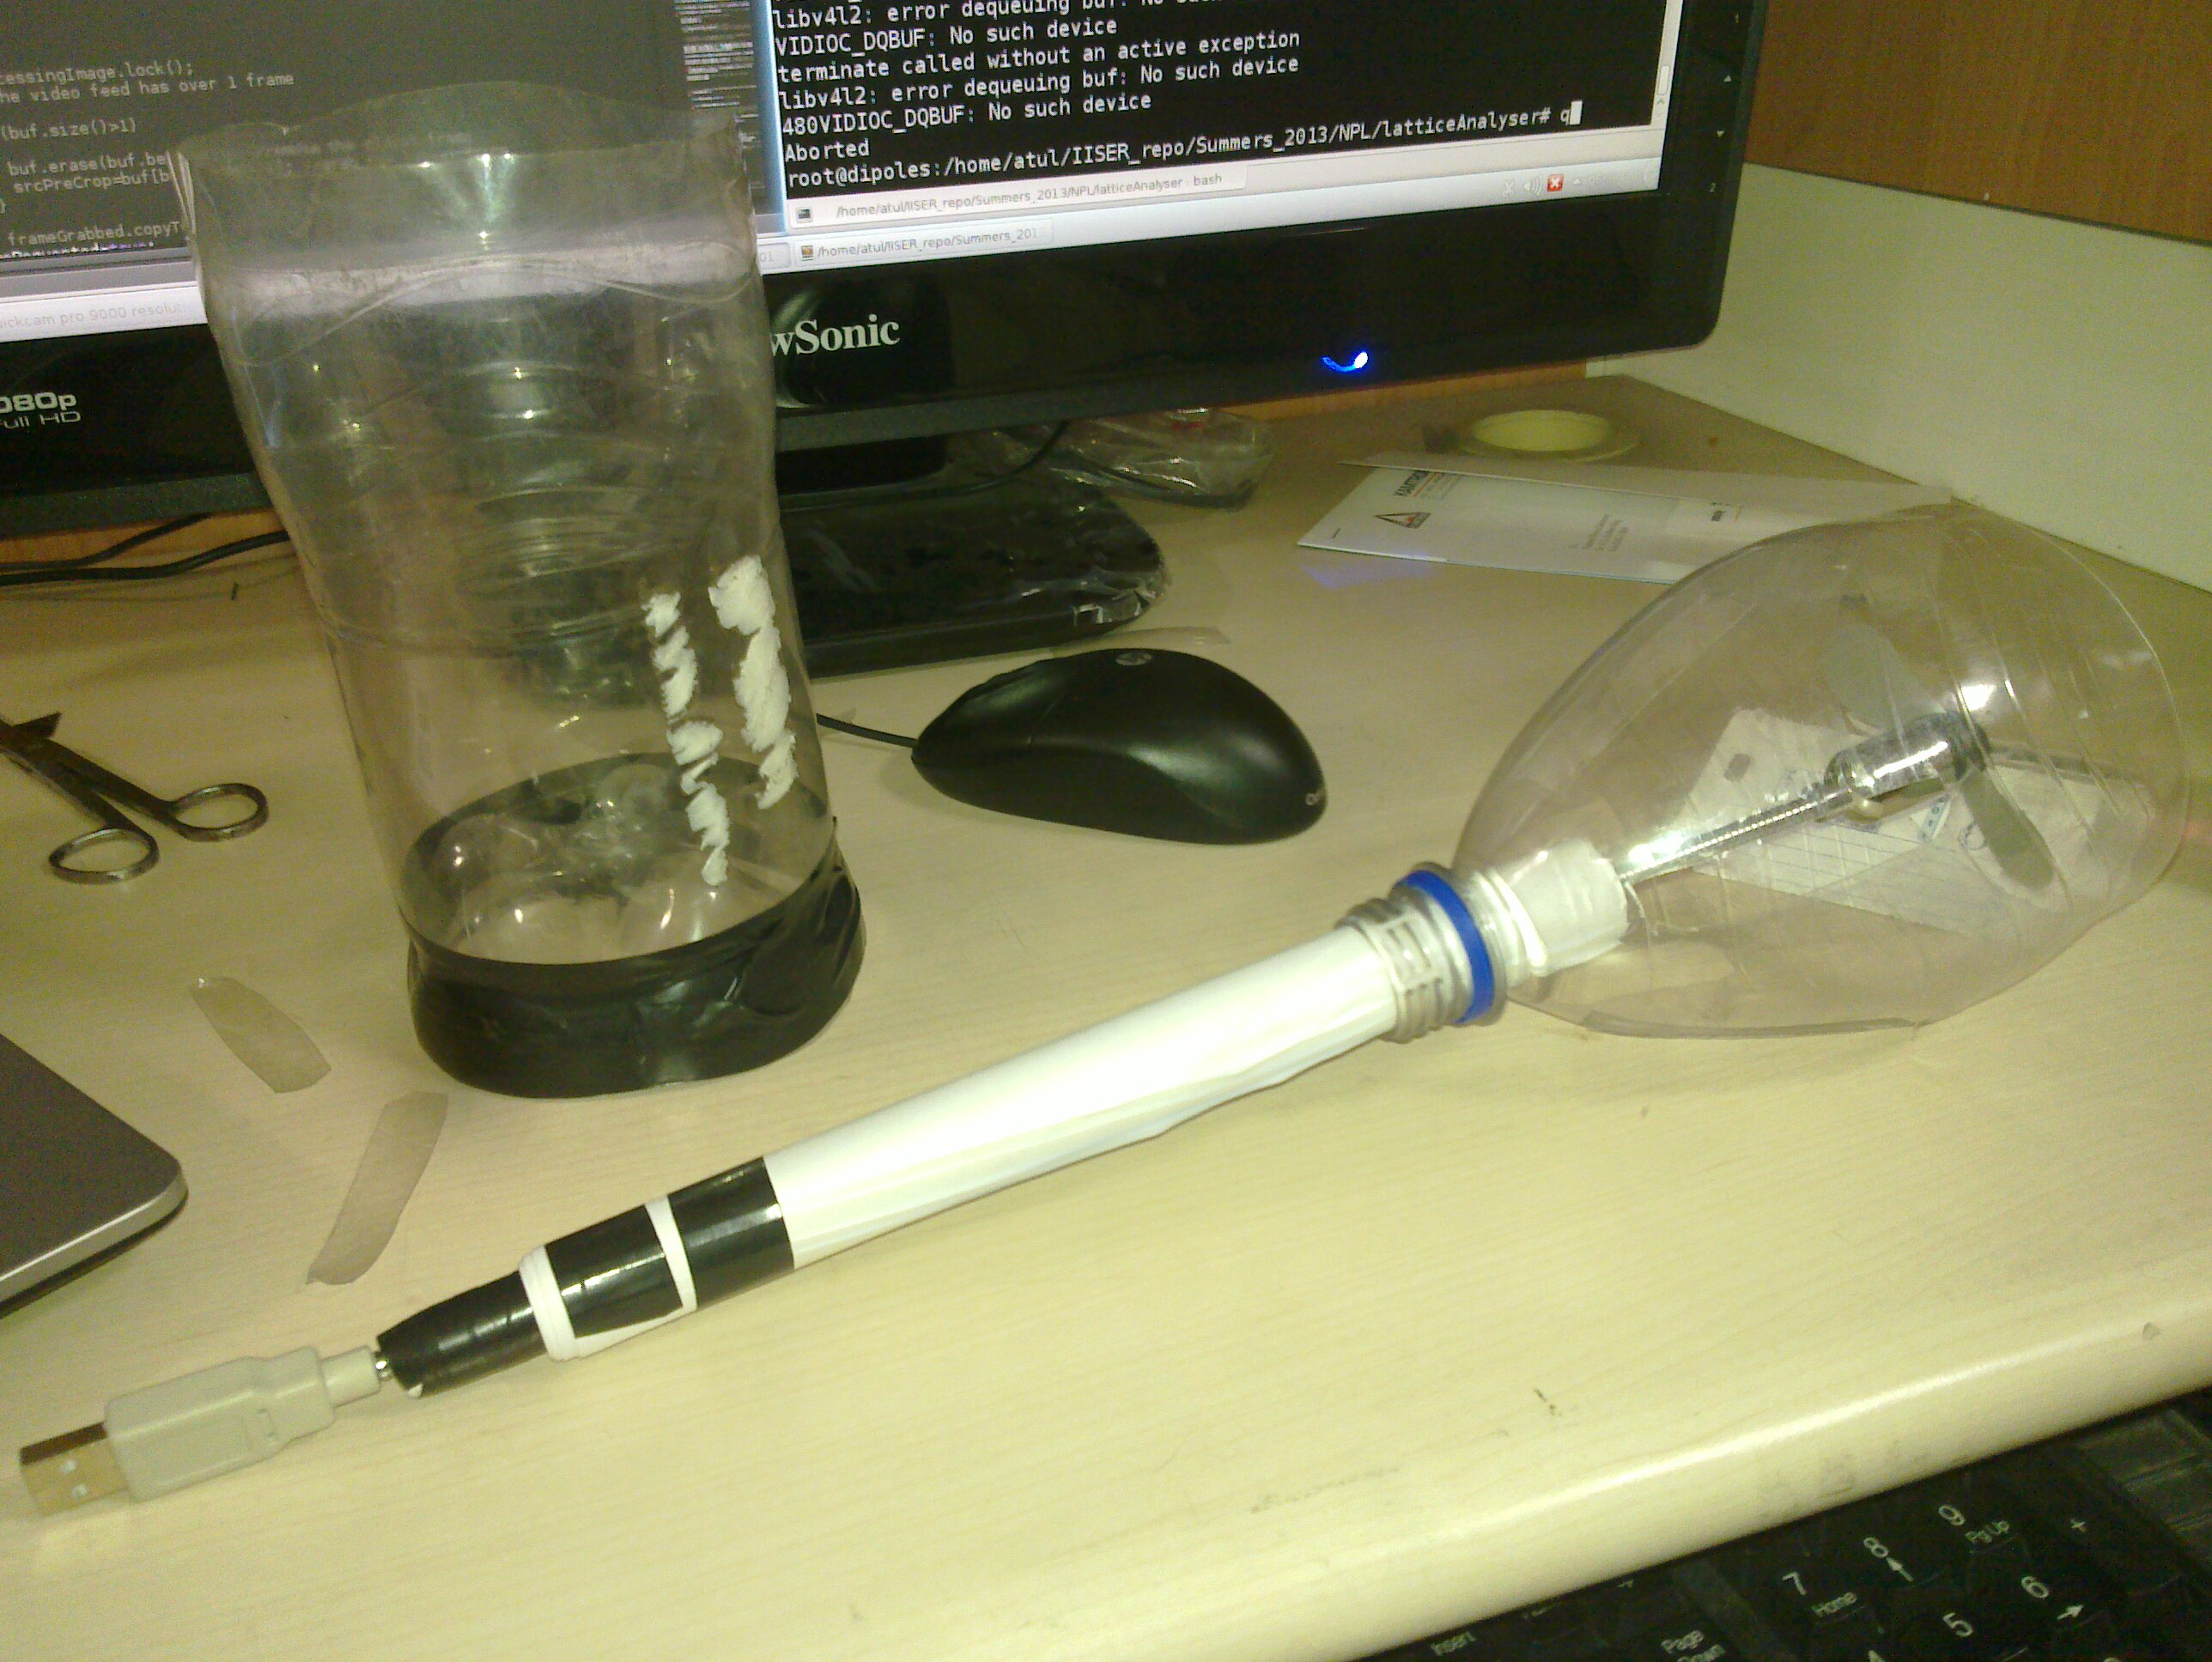
\includegraphics[width=0.7\linewidth]{gfx/fanSetupActual.jpg}
						\end{center}
					\caption[Final Fan Setup]{Final Fan Setup}
					\label{fanSetupActual}
					\end{figure}
					This failed miserably for the air pressure would fall the moment the assembly covered the fan. Introducing slits to allow air to flow in created no appreciable difference. This idea had to be dropped in favour of the vacuum cleaner setup as shown in \autoref{vacuumCleanerSetup}
					\begin{figure}[bth]
						\begin{center}
							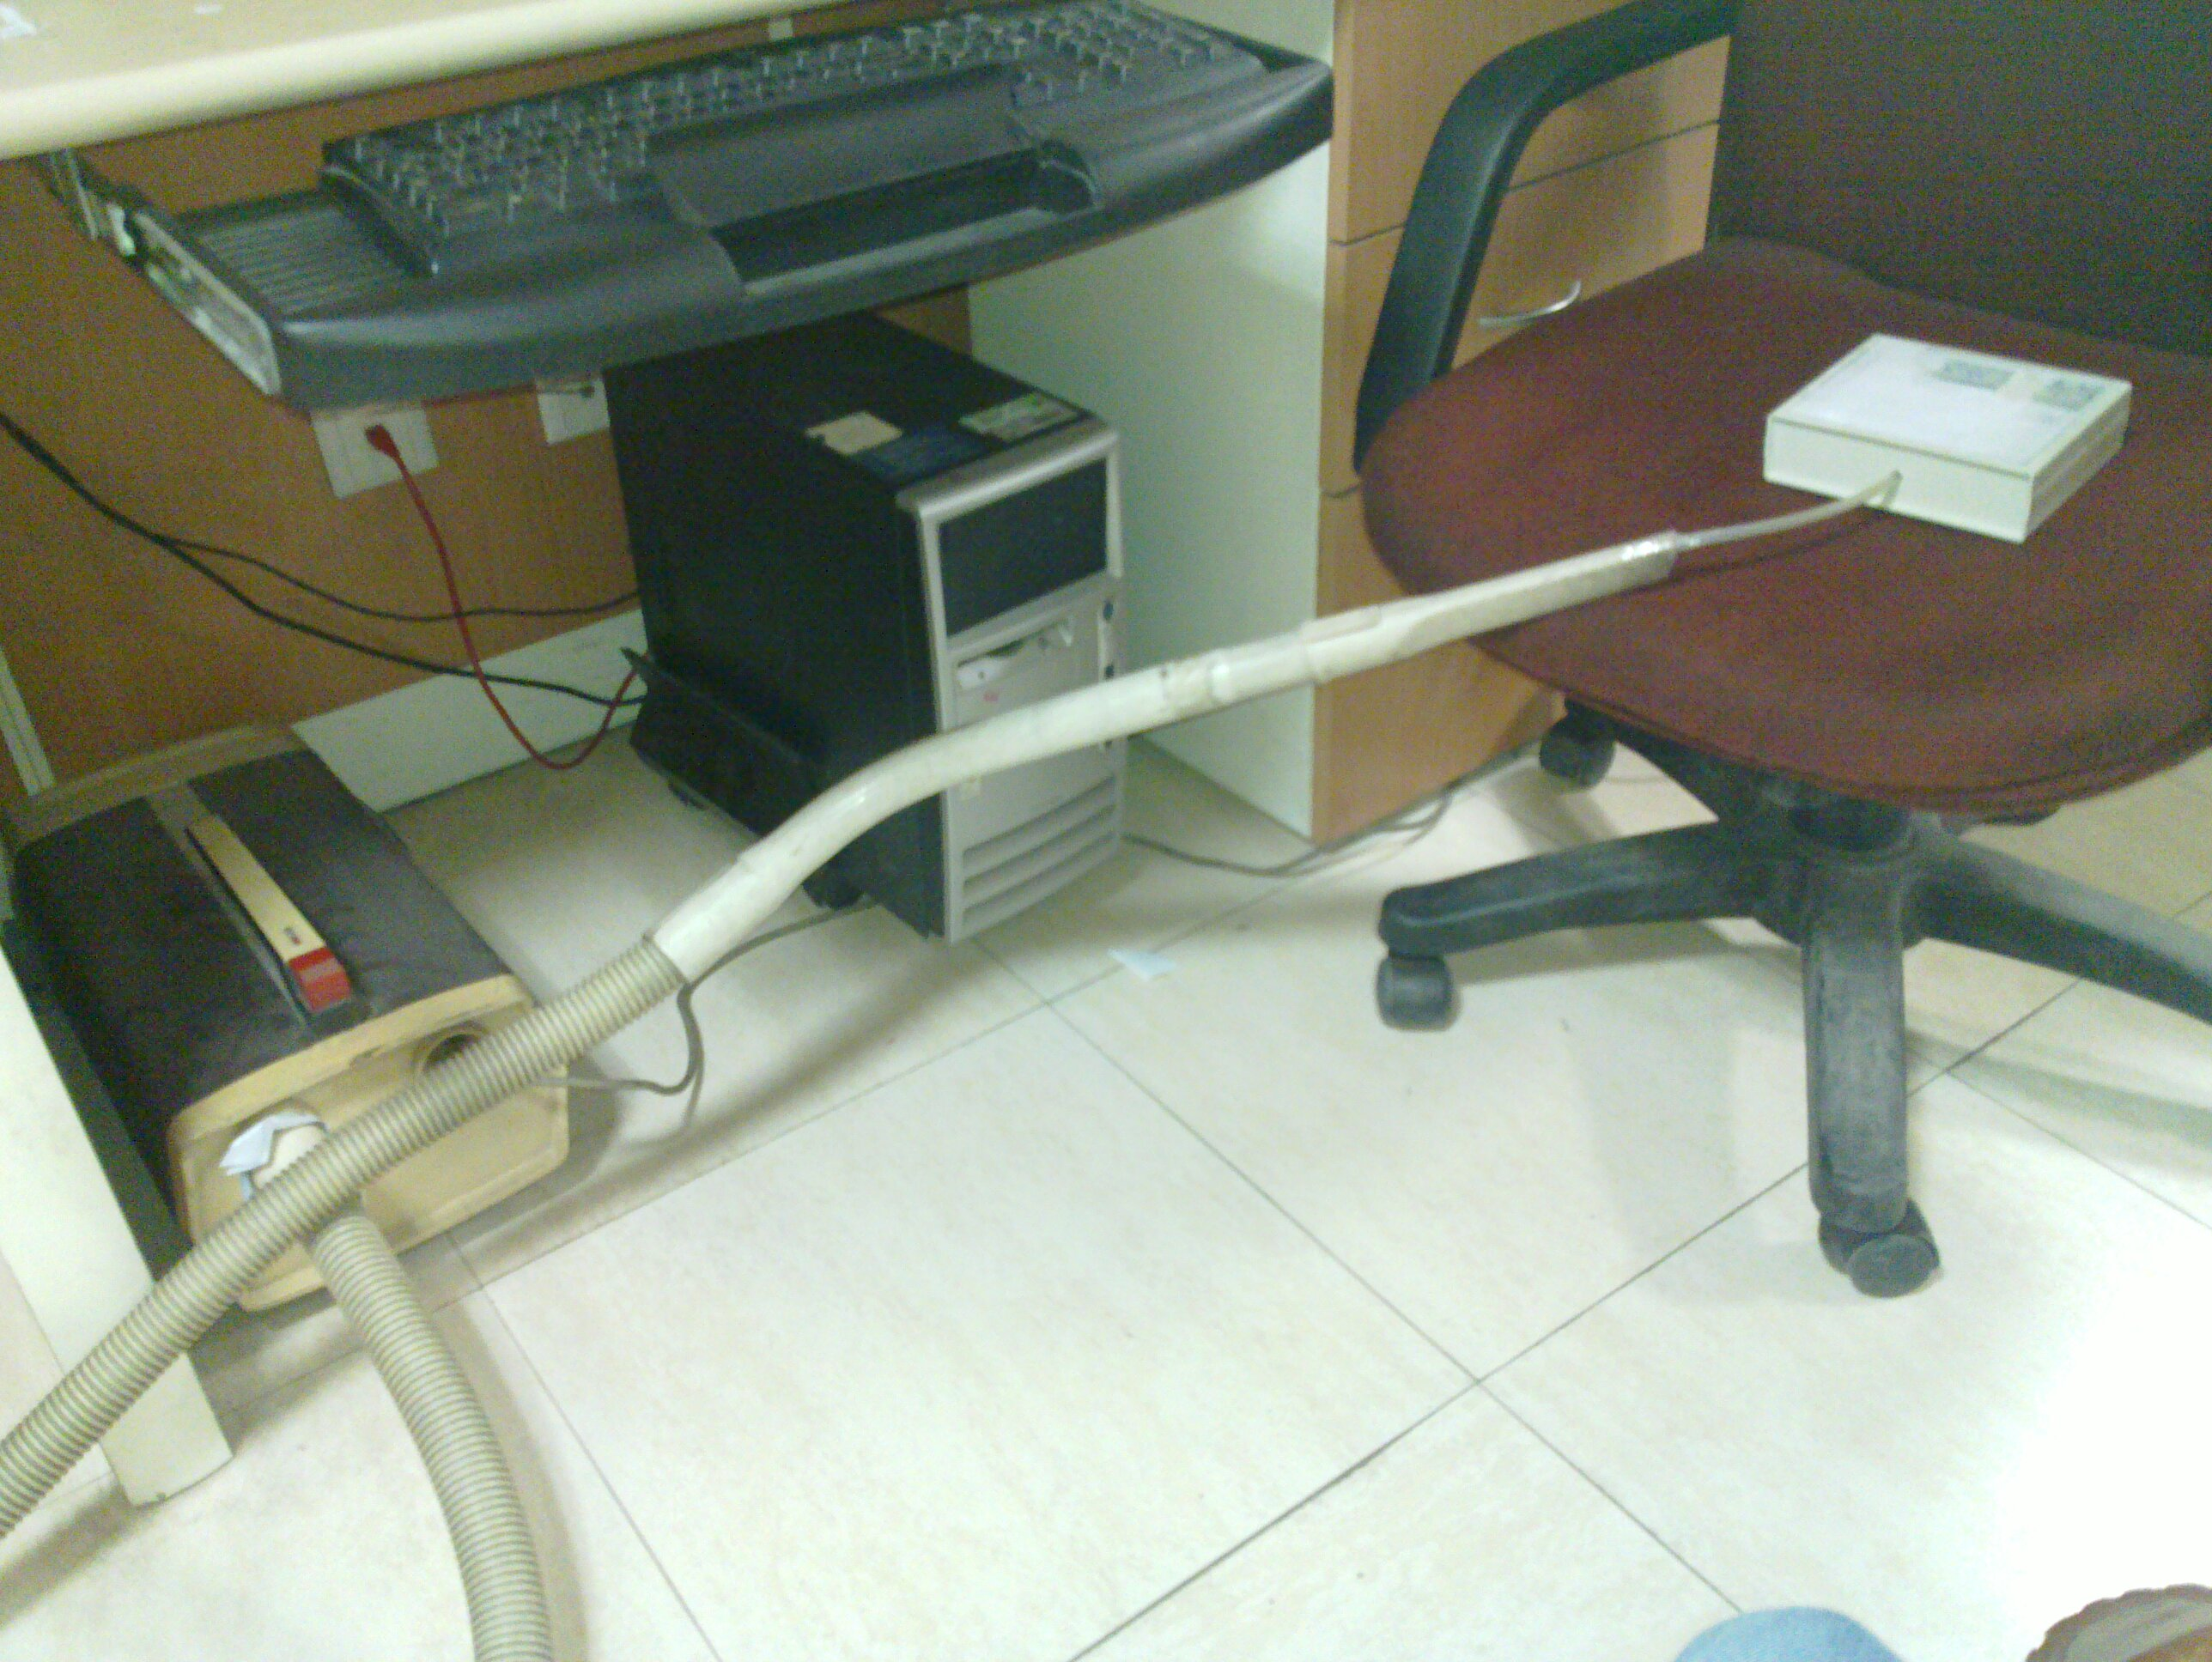
\includegraphics[width=0.7\linewidth]{gfx/vacuumCleanerSetup.jpg}
						\end{center}
					\caption[Vacuum Cleaner Setup]{Vacuum Cleaner Setup}
					\label{vacuumCleanerSetup}
					\end{figure}					 
					\par
					The vacuum cleaner was used as a blower and connected to a box using a pipe. On one of the faces of the box, four holes were drilled (which were later enlarged). These were covered to increase the pressure when required. On the open hole, one dipole was placed (which had to be re built with a minor modification, refer to \autoref{theLightDipole}) with a disc at the bottom. This is when an apparently bizarre observation was made. At a given pressure, it was found that the dipole could remain suspended in air beyond a certain height (and obviously there was an upper bound for the same). However, for heights lower than that, the dipole would fall. The explanation which seemed to resolve this was that the air could spread while rising sufficiently only beyond that height to apply pressure at a large enough surface area, thus create enough force. Albeit the experiment was not performed under precisely the same conditions, when it was repeated with a larger disc, the same problem was encountered, suggesting that there may be more to the explanation that deduced so far. Other geometries at the base (other than the disc) were also tried, such as a cone and a thermecol sphere, neither of which worked at low pressures which were enough to suspend the disc based setups. Further, at high pressures, disturbances in the form of torque in the dipole's axis of rotation begin to appear, which are fatal for the experiment.
					\begin{figure}[bth]
						\begin{center}
							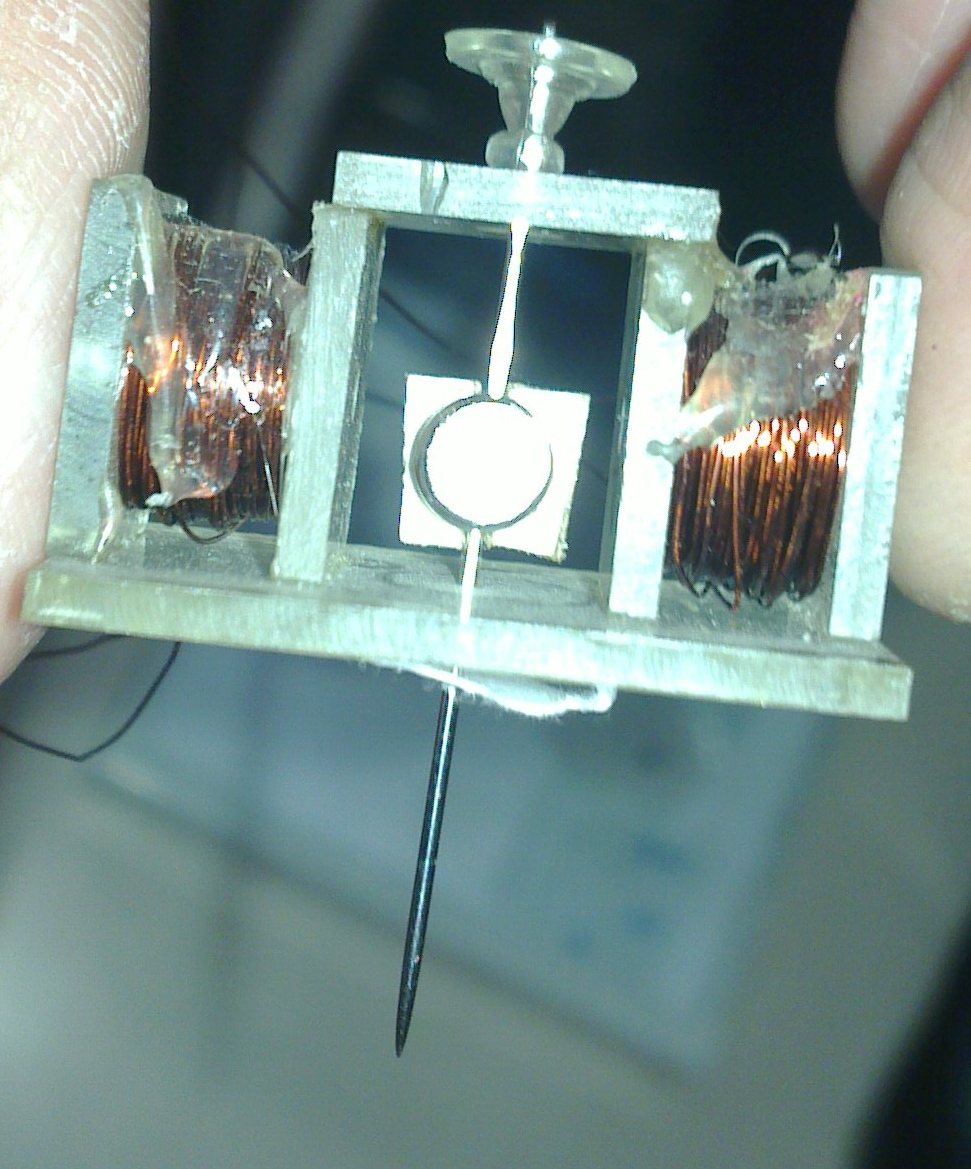
\includegraphics[width=0.7\linewidth]{gfx/theLightDipole.jpg}
						\end{center}
					\caption[The Modified Dipole]{The Modified Dipole}
					\label{theLightDipole}
					\end{figure}						
					\par
					Other problems with air-suspension included damping in the vertical direction. Once the dipole reaches the vertical equilibrium point, it overshoots just as an oscillator. Since the friction at the plates holding the needle vertical is negligible, the oscillations don't get damped quick enough. This was experimentally observed also. The energy ratio between the rotational part and the translation part, in the earth's field, was calculated and found to be approximately one for the given setup.
					\par
					The most stable we could achieve with this setup was using a cylindrical projection from which the high pressure air escapes and a disc of comparable size attached to the dipole. This did get suspended satisfactorily, unlike the other methods where the suspension could not be maintained at the desired height, however the needle became rather wobbly and unstable resulting in increased friction.
					\par
					Online research indicated that air-bearings do function well enough and so do the boards of air hockey. These will be explored in the coming weeks to improve upon the methods to achieve the desired results.
					\par
					THE DIPOLES
					\par
					Air hockey table method, DIY air hockey was a better method of searching, got cues
					\\
					aluminium disk's introduction (For air suspension), after finalizing one, and testing it, we found comparable resistance with the inverted needle top on glass slide as opposed to when air suspended. Hypothesised that the main source of friction was infact the guiding edges, which provide the opposing torque.
					\\
					an interesting setup was devised, with only the needle edges held using a glass slide and magnets. resist friction etc. 
					\\
					froze the design with aluminium disks at the bottom and made four good dipoles for testing in a 2x2 lattice
		\end{enumerate}
	\subsection{Construction of the Lattice Analyser}
		\subsubsection{Proof of Concept: Recognizing Patterns}
			The lattice analyser has come a long way. Image detection trials were initiated with \autoref{sampleImage}. 
			\begin{figure}[bth]
				\begin{center}
					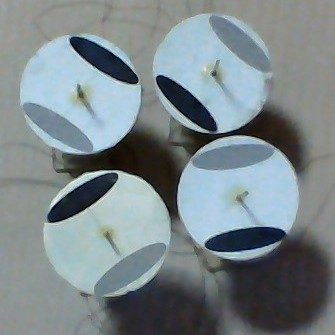
\includegraphics[width=0.7\linewidth]{../../latticeAnalyser/picture002.jpg}
				\end{center}
			\caption[Sample Image]{Sample Image}
			\label{sampleImage}
			\end{figure}

			The idea was that once the ellipses have been detected, and they are different in colour, one can evaluate from their centroids, the position and the angle of the dipole. It must be stated that earlier it was attempted to use the greyscale image as was provided. However soon the shadow interference led to using coloured patterns instead. These patterns were not printed but displayed on a screen and the camera aimed appropriately.
			\par
			So first, the algorithm for detection of relevant part of the image had to be frozen. There were two candidates for this
			\begin{enumerate}
				\item Hough Transform Method
					\par
					Either one could use the already available in OpenCV, line detection or circle detection, both would've required changing the pattern on the dipole
					\par
					Or one could use an ellipse modification for the same, which would require programming the algorithm.
				\item Contour Detection and Ellipse Fitting
					\par
					This method detects contours in a given image, and the OpenCV example also shows ellipse fitting for the same. This seemed promising too, but it seemed more expensive (computationally) than looking for predetermined shapes.
			\end{enumerate}
			This work had been done within the first few days. 
			\par

			\begin{figure}[bth]
				\begin{center}
					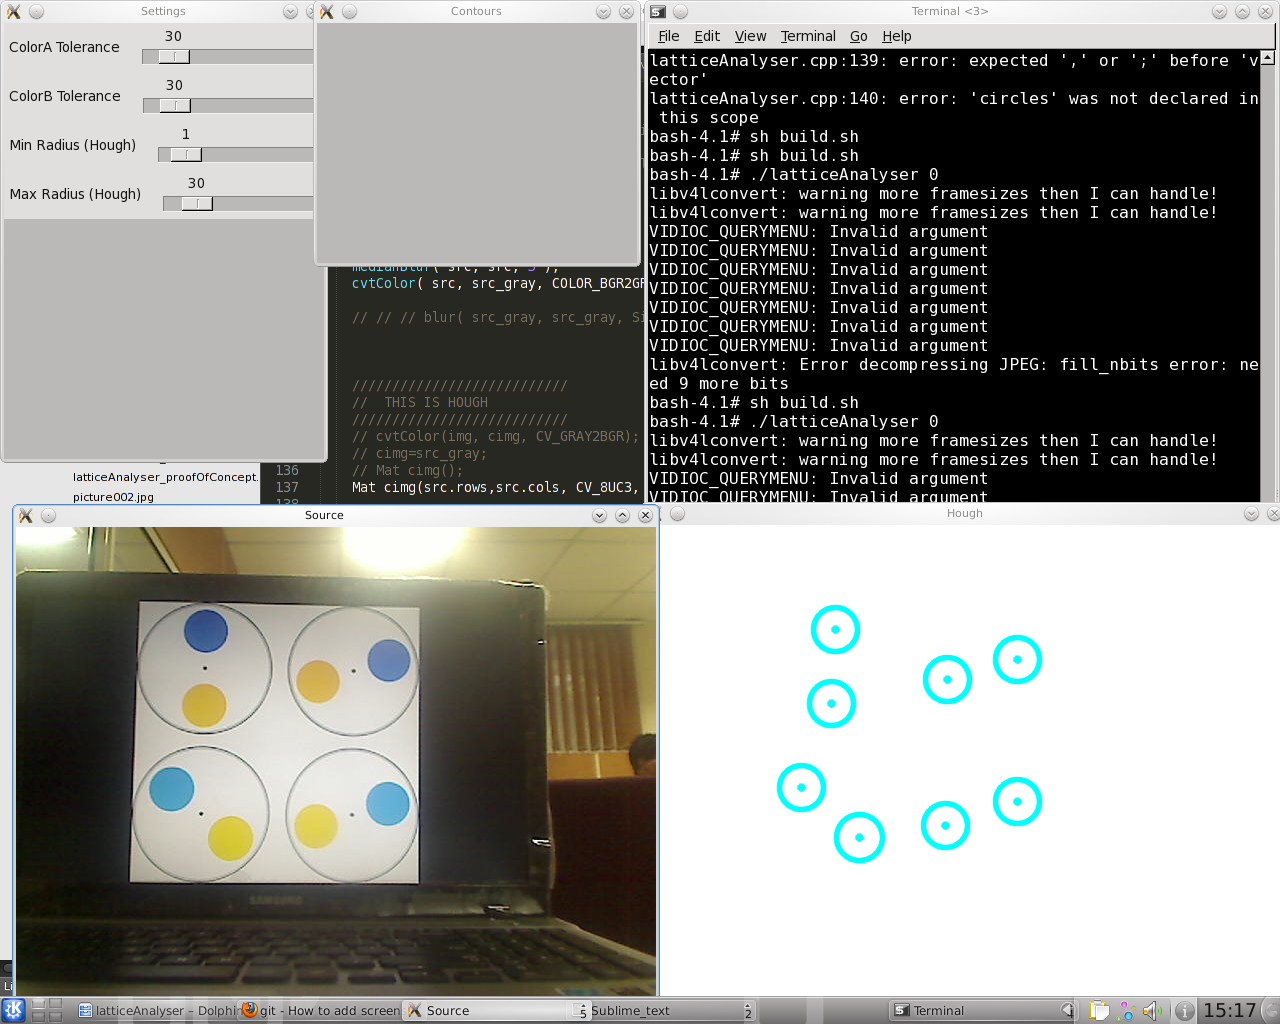
\includegraphics[width=1.1\linewidth]{../../latticeAnalyser/snapshot1.png}
				\end{center}
			\caption[Hough Transform]{Hough Transform}
			\label{snapshot1}
			\end{figure}

			\begin{figure}[bth]
				\begin{center}
					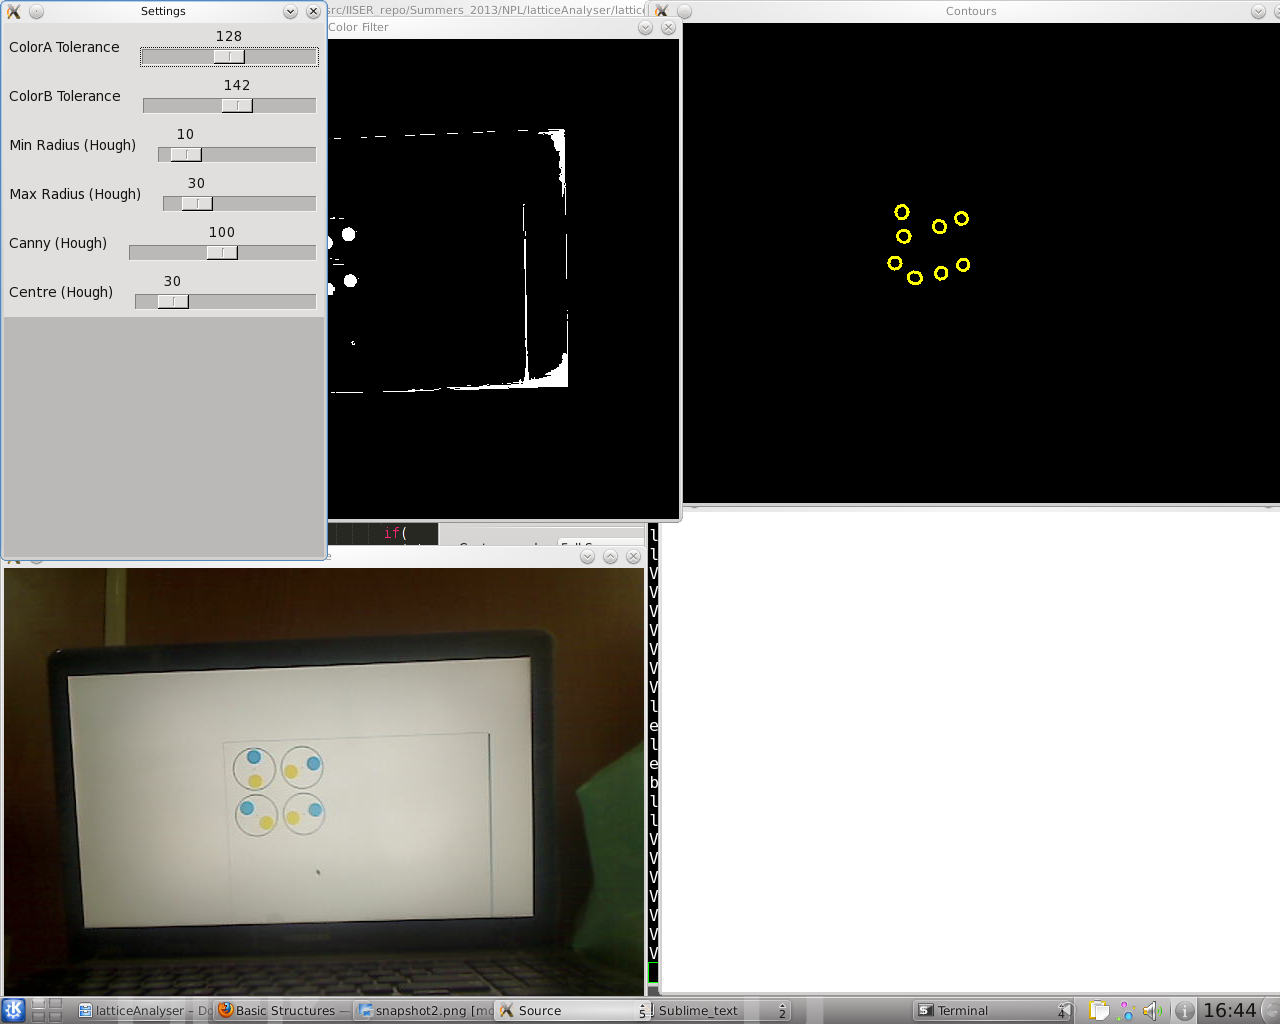
\includegraphics[width=1.1\linewidth]{../../latticeAnalyser/snapshot2.png}
				\end{center}
			\caption[Contour Detection]{Contour Detection}
			\label{snapshot2}
			\end{figure}

			Next, a colour filter was to setup to improve the accuracy. When the algorithms were implemented, it was found that the Hough Transform method often misses detection of circles, refer to \autoref{snapshot1} (this is ofcourse after attaching a video stream instead of images to the code) as compared to contour detection \autoref{snapshot2}.
			\par

			\begin{figure}[bth]
				\begin{center}
					
\includegraphics[width=0.3\linewidth]{../../latticeAnalyser/singleDipole.png}
				\end{center}
			\caption[Final Pattern]{Final Pattern}
			\label{singleDipole}
			\end{figure}

			\begin{figure}[bth]
				\begin{center}
					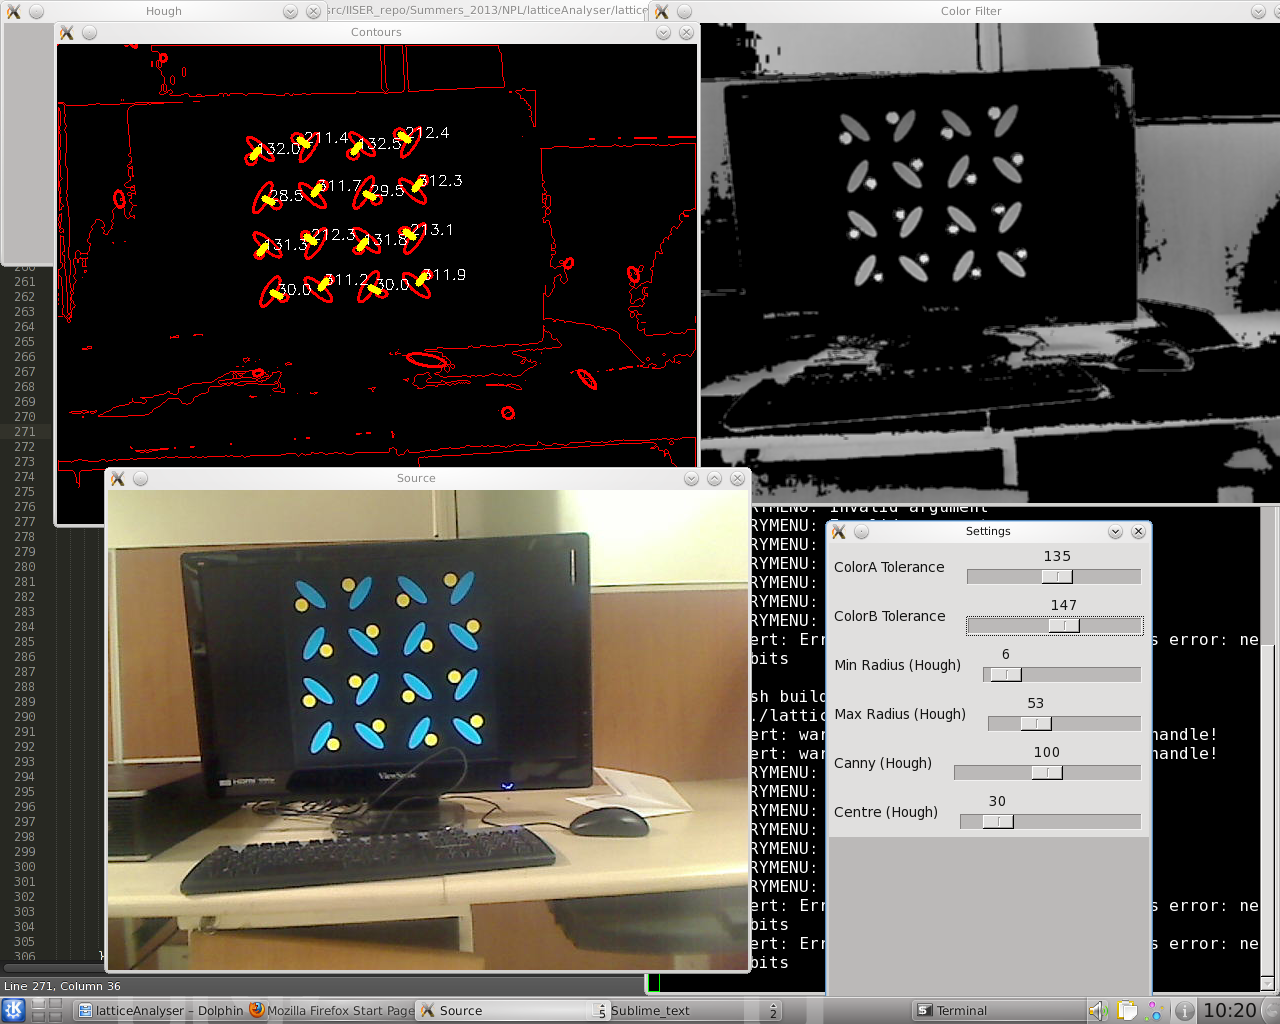
\includegraphics[width=1.1\linewidth]{../../latticeAnalyser/snapshot5.png}
				\end{center}
			\caption[Multi Shape, Single Colour]{Multi Shape, Single Colour}
			\label{snapshot5}
			\end{figure}

			After the detection, according the plan, two colours were to be used for the ellipses. However, running the hough transform twice would've dropped the detection speed to half, which wasn't worth it. It was then decided that the shapes should be made different instead of relying on two colours for the same information. After looking at various combinations, \autoref{singleDipole} was finalized, with an ellipse at the centre, and a circle along the minor axis for breaking the symmetry. This method did infact work as shown in \autoref{snapshot5}.
			\par

			\begin{figure}[bth]
				\begin{center}
					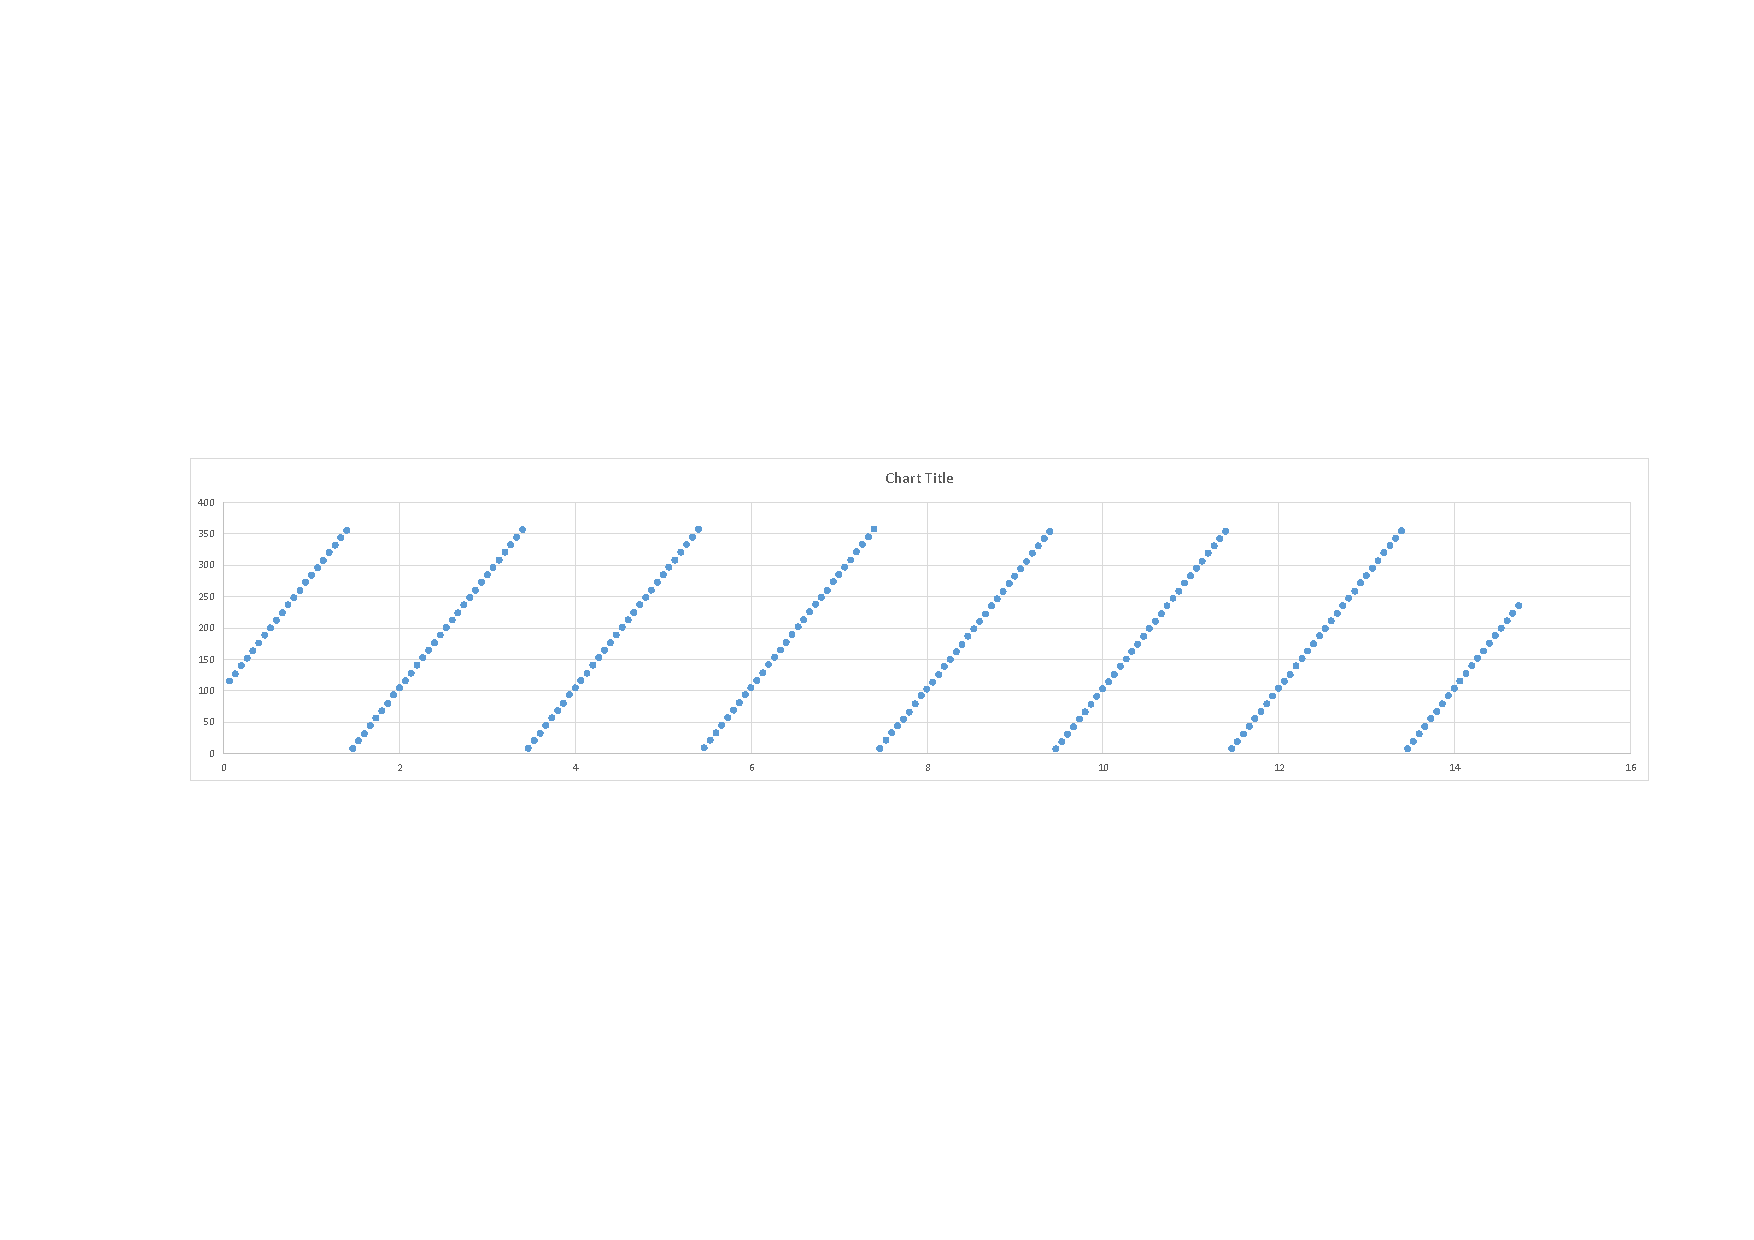
\includegraphics[width=1.1\linewidth]{../../latticeAnalyser/testGraphs}
				\end{center}
			\caption[First Observation]{First Observation}
			\label{testGraphs}
			\end{figure}
		\subsubsection{Aftermath and Recognition Tests}
			The next challenge was to realize that a dipole detection can be missed and therefore mess up the counting, if that is the only way of uniquely identifying them. Unique identification is obviously required, as the external hardware must fire the coils of the right dipole. Thus a reference frame was used to uniquely identify the dipoles initially. This is expected to happen when they are stationary to get a good reading. In each frame, whenever a dipole is detected, it is associated with the dipole in the reference frame, by matching its location. If a dipole is not detected in a given frame, the software knows it was unable to record it and doesn't mess up neither the numbering nor the observations.
			\par

			\begin{figure}[bth]
				\begin{center}
					
\includegraphics[width=0.7\linewidth]{../../latticeAnalyser/ellipseCircleDipoles4x4_black.jpg}
				\end{center}
			\caption[Final Test Pattern]{Final Test Pattern}
			\label{testPattern}
			\end{figure}

			After implementation of the last part, an animation sequence was created in Power Point, with the dipoles rotating with a constant speed and the camera was aimed at the screen. A still from the same is given in \autoref{testPattern}. \autoref{testGraphs}, shows the angular position versus time plot, for the first dipole and yes, it is linear, just as expected. Standard deviation tests are still to be done.
			\par
			Further tests, relating to it's timing were done and it was found that the processing itself was taking longer than the time taken by one frame in a 30 FPS video stream. This could be improved with the following
			\begin{enumerate}
				\item Intel Performance Primitives (IPP)
					\par
					These are libraries that provide optimized algorithms for performing some of the basic tasks in OpenCV to speed up the overall computation
				\item Multi Threading
					\par
					Rendering the frames in a different thread could perhaps increase the render speed or atleast ensure it doesn't affect the rate of processing of the image
				\item Camera Initial Delay
					\par
					Despite a 30 FPS smooth video, there seemed to be an initial delay which persisted in the video preview of the camera. This can be corrected for by polling the camera quickly instead of processing the image each time.
				\item OpenTBB
					\par
					To enable multi-threading within OpenCV to speed up the algorithms
				\item Hardware
					\par
					The results obtained earlier were for a Pentium 4 HT system. A faster multi-core processor could produce potentially, better benchmarks.
			\end{enumerate}
			Painstakingly, IPP was downloaded, built and integrated with OpenCV and re-built. There were various issues, starting from an incompatible version of IPP, to faulty documentation in OpenCV. The results did not improve however despite this. Perhaps the algorithms used do not rely on the methods optimized by IPP
			\par
			Multi-threading was implemented using C++ 11. Various synchronization methods were looked up, including mutexes, uniqe locks; eventually atoms were used and tested with Visual Studio Express 2012 on windows (implicitly implying the application was first made to run on windows), as the linux machine had an older kernel and upgrading GCC wasn't recommended.
			\par
			The camera's initial delay is caused by the initial stream. To rectify this, OpenCV has two methods, one for grabbing a frame, and the other for decoding it. If in a separate loop, the camera is polled regularly for frames, the delay is minimized. The frame can be decoded as soon as processing of the previous frame is over. This, as is suggestive, also requires multi-threading
			\par
			OpenTBB is a library that is required to enable multi-threading support in OpenCV. This too had to be fiddled with for a while, before being built successfully.
			\par
			The hardware was changed to an i7 machine which has more then enough cores and computation power.
			\par
			These modifications were all combined and the code compiled using GCC (except certain parts of multi-threading, due to a compiler issue) and it was found to be able to process in about 25 milliseconds for an $8 \times 8$ matrix of dipoles. For a $16 \times 16$ matrix, the resolution of the camera (Logitech Pro 9000, $640 \times 480$ at 30 FPS) was found to be insufficient. Higher resolutions in the same camera did not have a 30 FPS temporal resolution. The alternative seems to be a camera for the Rasberry Pi which can be used over ethernet.
			\par
			Further, the CLI of the program was modified to add support for inputting various commands, which would be required for testing the hardware (which is scheduled to be built this week).
		\subsubsection{`temperature' compatible}
			\par
			And surprise surprise, the hardware interface was in fact done in the following week. \myProf had already created a simplified version of the Ob-Dev firmware for USB interface of an Atmega with the PC which was used. More on that is there in the temperature section (which follows). The Lattice Analyser had to pump in energy to the system by providing angular velocity to the system of dipoles repetitively at suitable time intervals, viz. when the temperature of the system drops. The temperature is calculated in realtime using the RMS angular velocity of each dipole in the system. It was immediately realized after a closer look that since the time window between two frames is roughly 30 ms, it is not possible to energize all the dipoles with velocities picked from a given distribution of temperature. Further, since the motion of the entire system is coupled, it suffices to energize \emph{some} dipoles sufficiently to maintain the temperature.
			\par
			To achieve this the following were done (or algorithms for achieving them written) \footnote{For completeness sake, it must be stated that some modifications had to be made before the colour filtration became functional}
			\begin{enumerate}
				\item The tools for compiling and programming the AVR installed
				\item Bootloader programmed into the micro-controller along with the sample program given by \myProf
				\item Communication with the PC was tested using the corresponding C example program for the PC
				\item USB libraries were incorporated into the latticeAnalyser and linked (had to compile C objects with C++ objects)
				\item A simple IO protocol between the Lattice Analyser and the microcontroller was written and tested.
				\item The coil of a dipole was tested with a set of 4 A4 batteries and some basic current calculations were done
				\item The hardware was setup to include a small current limiting resistor (about 120 ohms) and the coil powered using the Lattice Analyser
				\item (was not required) Worked on sachetIO; a library for breaking down a large chunk of data into sachets intended to be transmitted and combined after being received.
				\item (was not required) Looked up methods to amplify the current, since the micro-controller's current wasn't found to be strong enough to align the needle of the dipole to it.
				\item Discussion about how to implement the energy pumping (which is how the previous two steps were found to be pointless)
				\item A $2 \times 2$ lattice of dipoles was setup. 
				\item The angular velocities of each dipole calculated
				\item With each frame, the RMS angular velocity calculated
				\item An algorithm for position and velocity based energy pumping written
				\item Interface added to test the same by supporting inversion of force direction (so that it results in halting) and an option to make blind (viz. disable the algorithm and instead send pulses periodically in time)
			\end{enumerate}
			The final result was that energy could be pumped into one dipole satisfactorily. The next step was to extend the algorithm to an arbitrarily sized matrix. Certain steps such as velocity calculations when dipole detection fails (at high speeds) has arbitrary inaccurate behaviour in the said version. Algorithms for finding the axis of the coil in the dipoles also needs to be finalized, for there are more than one ways of doing this, viz. powering the coils and reading the angular position of the dipole, finding the axis of the lattice by noting the Cartesian positions of the dipole, deduce it from the rest (initial) angular position of the dipoles which should be known given the lattice size, etc.				
		\subsubsection{Adding Realtime Graphing Capability}
			Before working further on the aforesaid steps, realtime graphing was implemented. This was thought to be required for \emph{seeing} what was happening, specially the angle detection and when it goes wrong. This is being emphasized because the angle detection would often result in incorrect angle calculation which was a serious issue.
			\par
			After searching the internet for plotting methods, plplot was finalized as the graphing library to be used with C++. This was downloaded, built and installed. I wouldn't go into the implementation details, but would remark that it takes a little time to get everything up and running. The library supports various kinds of graphs. The two types of that were used for the project are
			\begin{enumerate}
				\item Realtime 3D plot
				\item Strip chart
			\end{enumerate}
			Further, the library provides multiple rendering options, of which for linux, a driver for the x11 graphics system was used for testing. In a single window all three graphs were created;
			\begin{enumerate}
				\item 3D: Angular Position vs Dipole ID vs Time
				\item 3D: Angular Velocity vs Dipole ID vs Time
				\item Stripchart: Average Square Angular Velocity (over dipoles) vs Time
			\end{enumerate}
			Of course, these graphs weren't all added at once; \autoref{snapshot8}, \autoref{snapshot9} and \autoref{snapshot11} tell the story. For the stripchart it must be remarked that it auto scales and shifts as the data flows in. This proved to be more useful than expected for debugging the mod problem (helped visually see the co-relation between other parameters and occurrence of the error). Further it was also useful in identifying periodic fluctuations (with a somewhat constant time period) in the third graph.
			\begin{figure}[bth]
				\begin{center}
					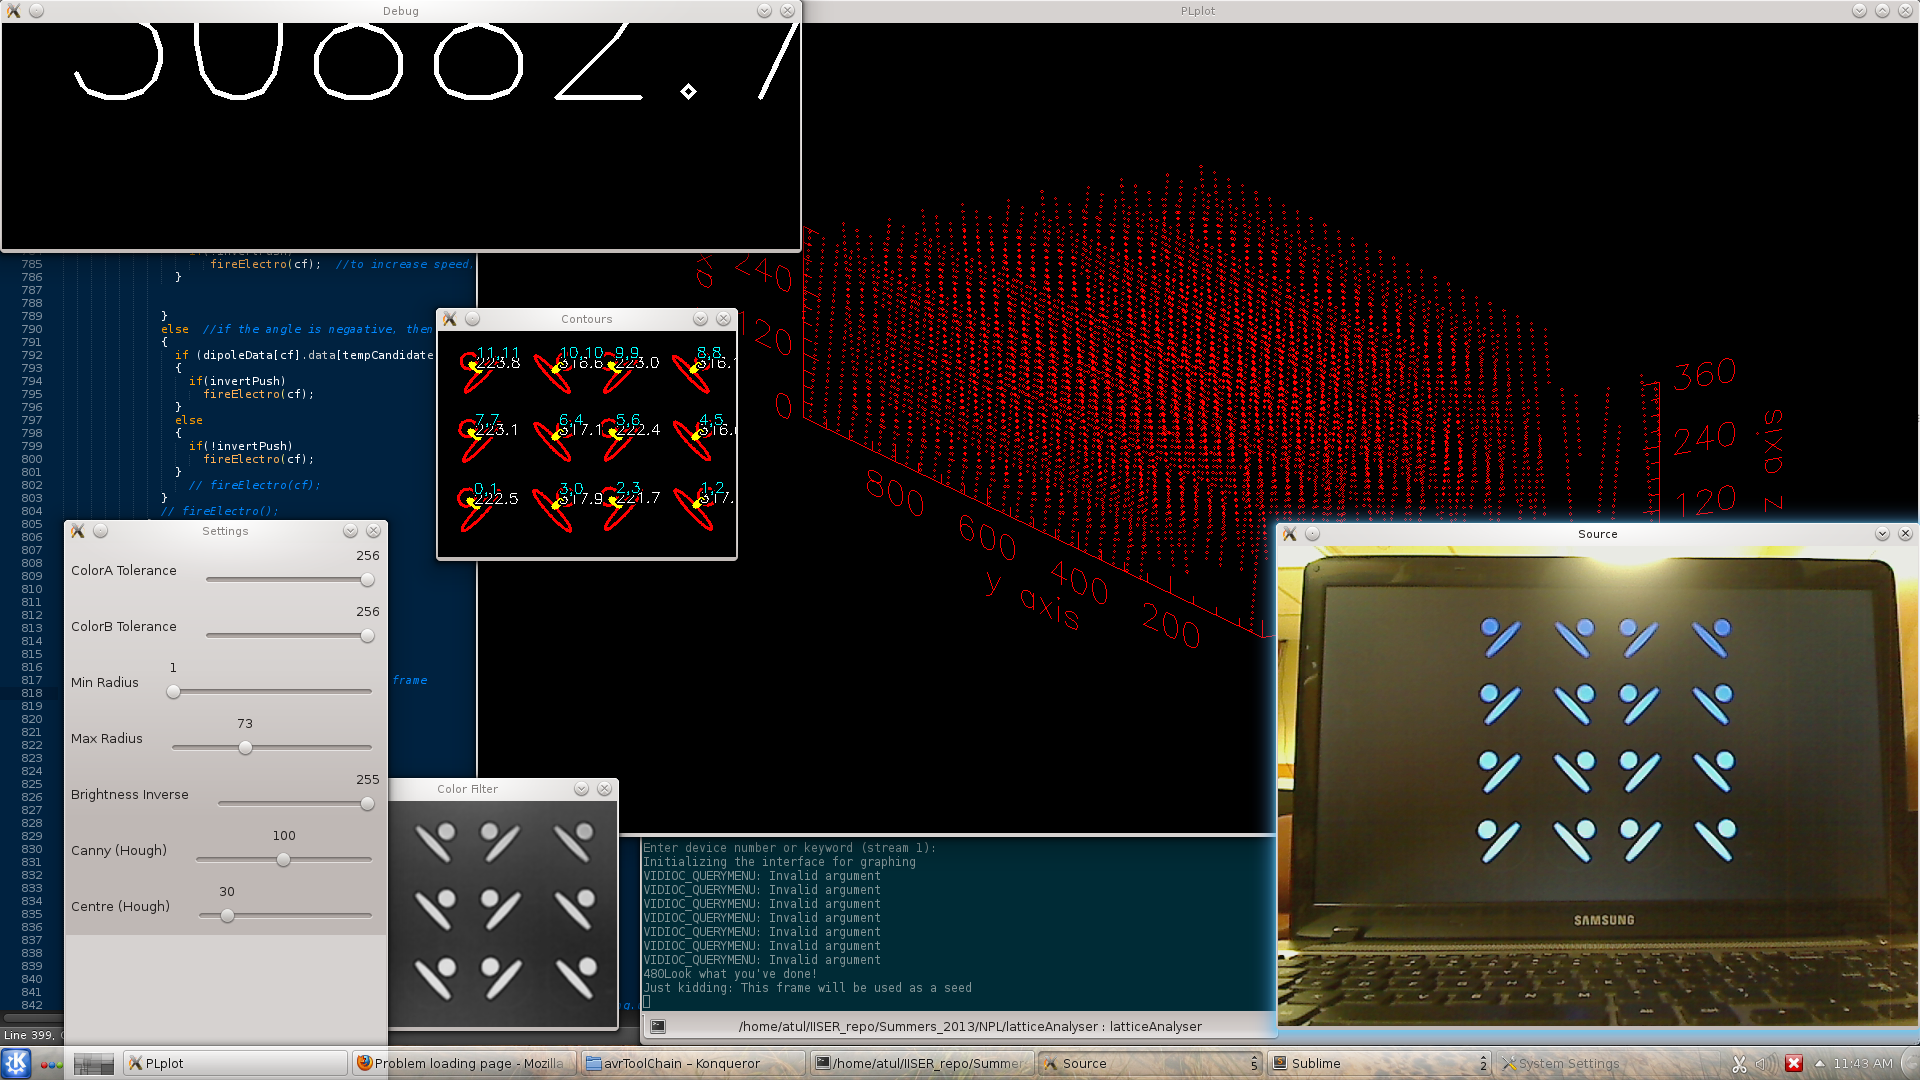
\includegraphics[width=1.1\linewidth]{../../latticeAnalyser/snapshot8.png}
				\end{center}
			\caption[With the first graph]{With the first graph}
			\label{snapshot8}
			\end{figure}

			\begin{figure}[bth]
				\begin{center}
					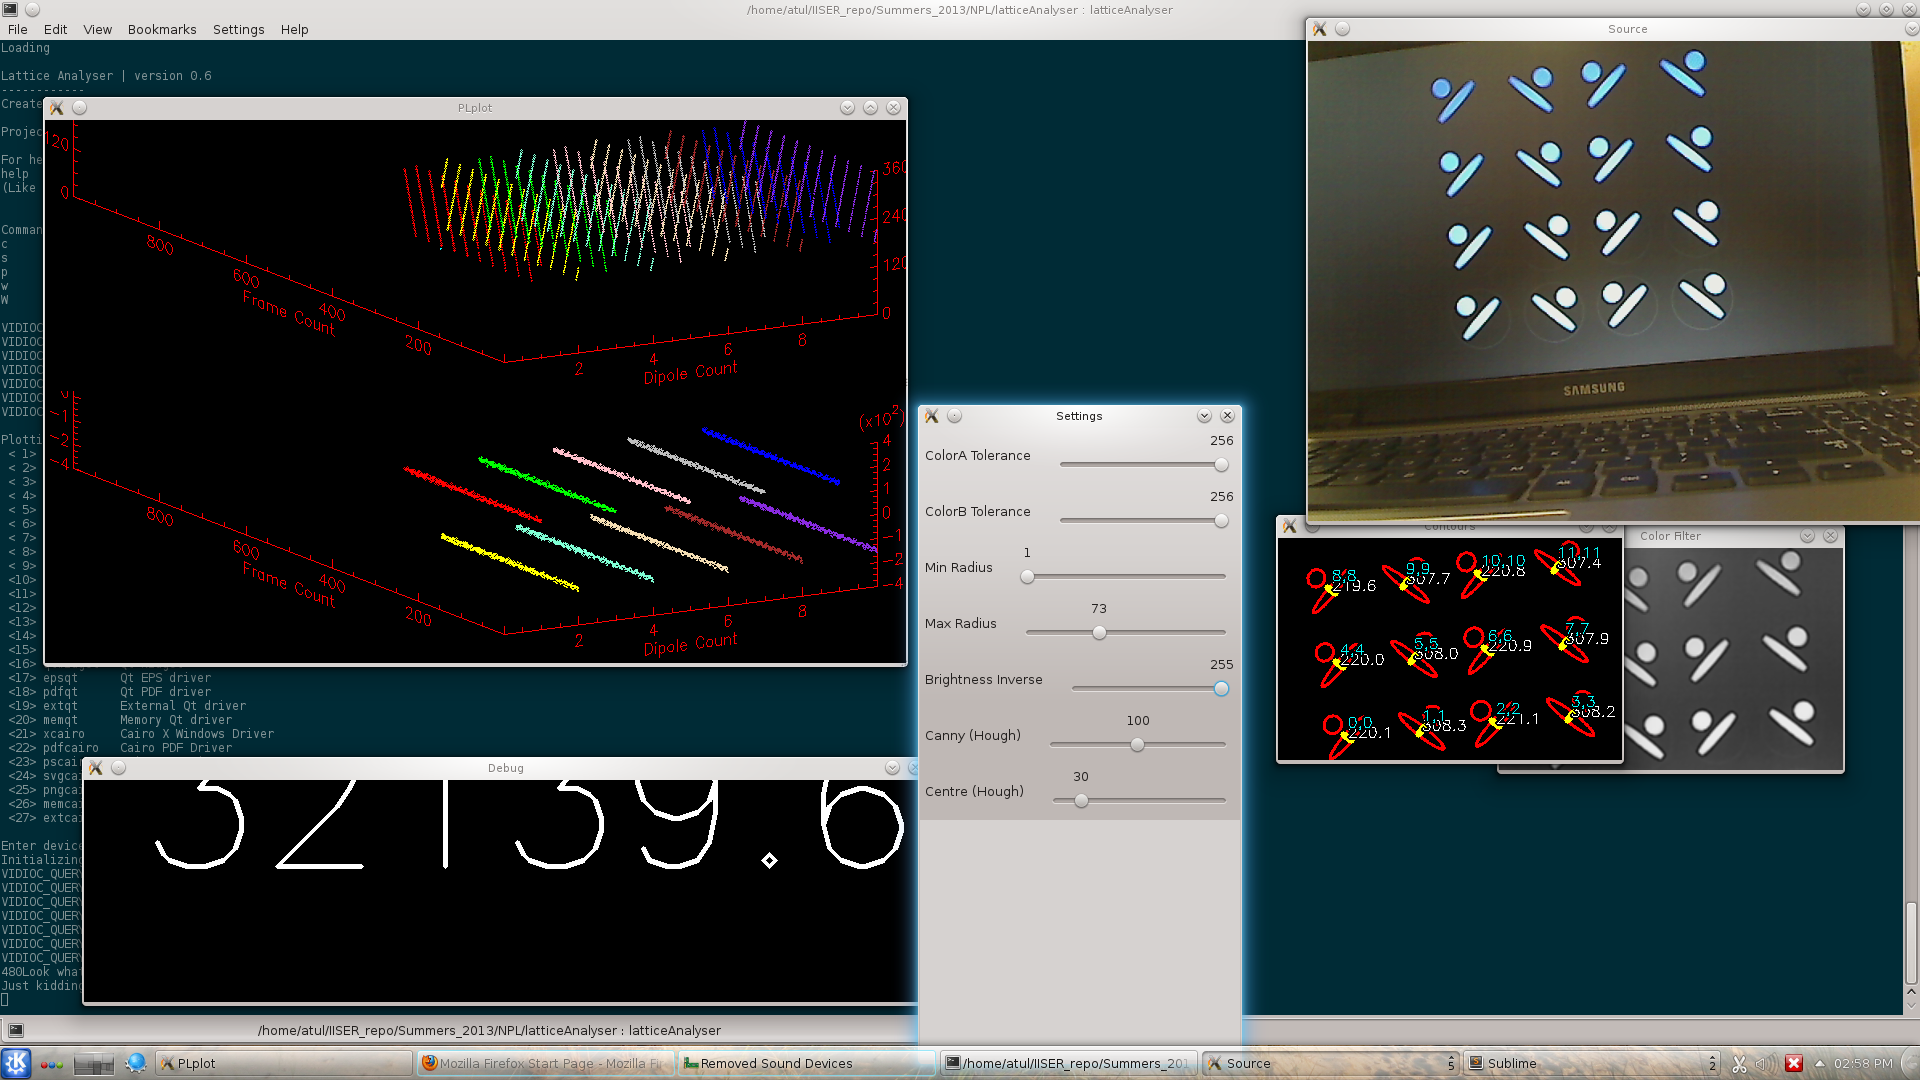
\includegraphics[width=1.1\linewidth]{../../latticeAnalyser/snapshot9.png}
				\end{center}
			\caption[With the second graph]{With the second graph}
			\label{snapshot9}
			\end{figure}

			\begin{figure}[bth]
				\begin{center}
					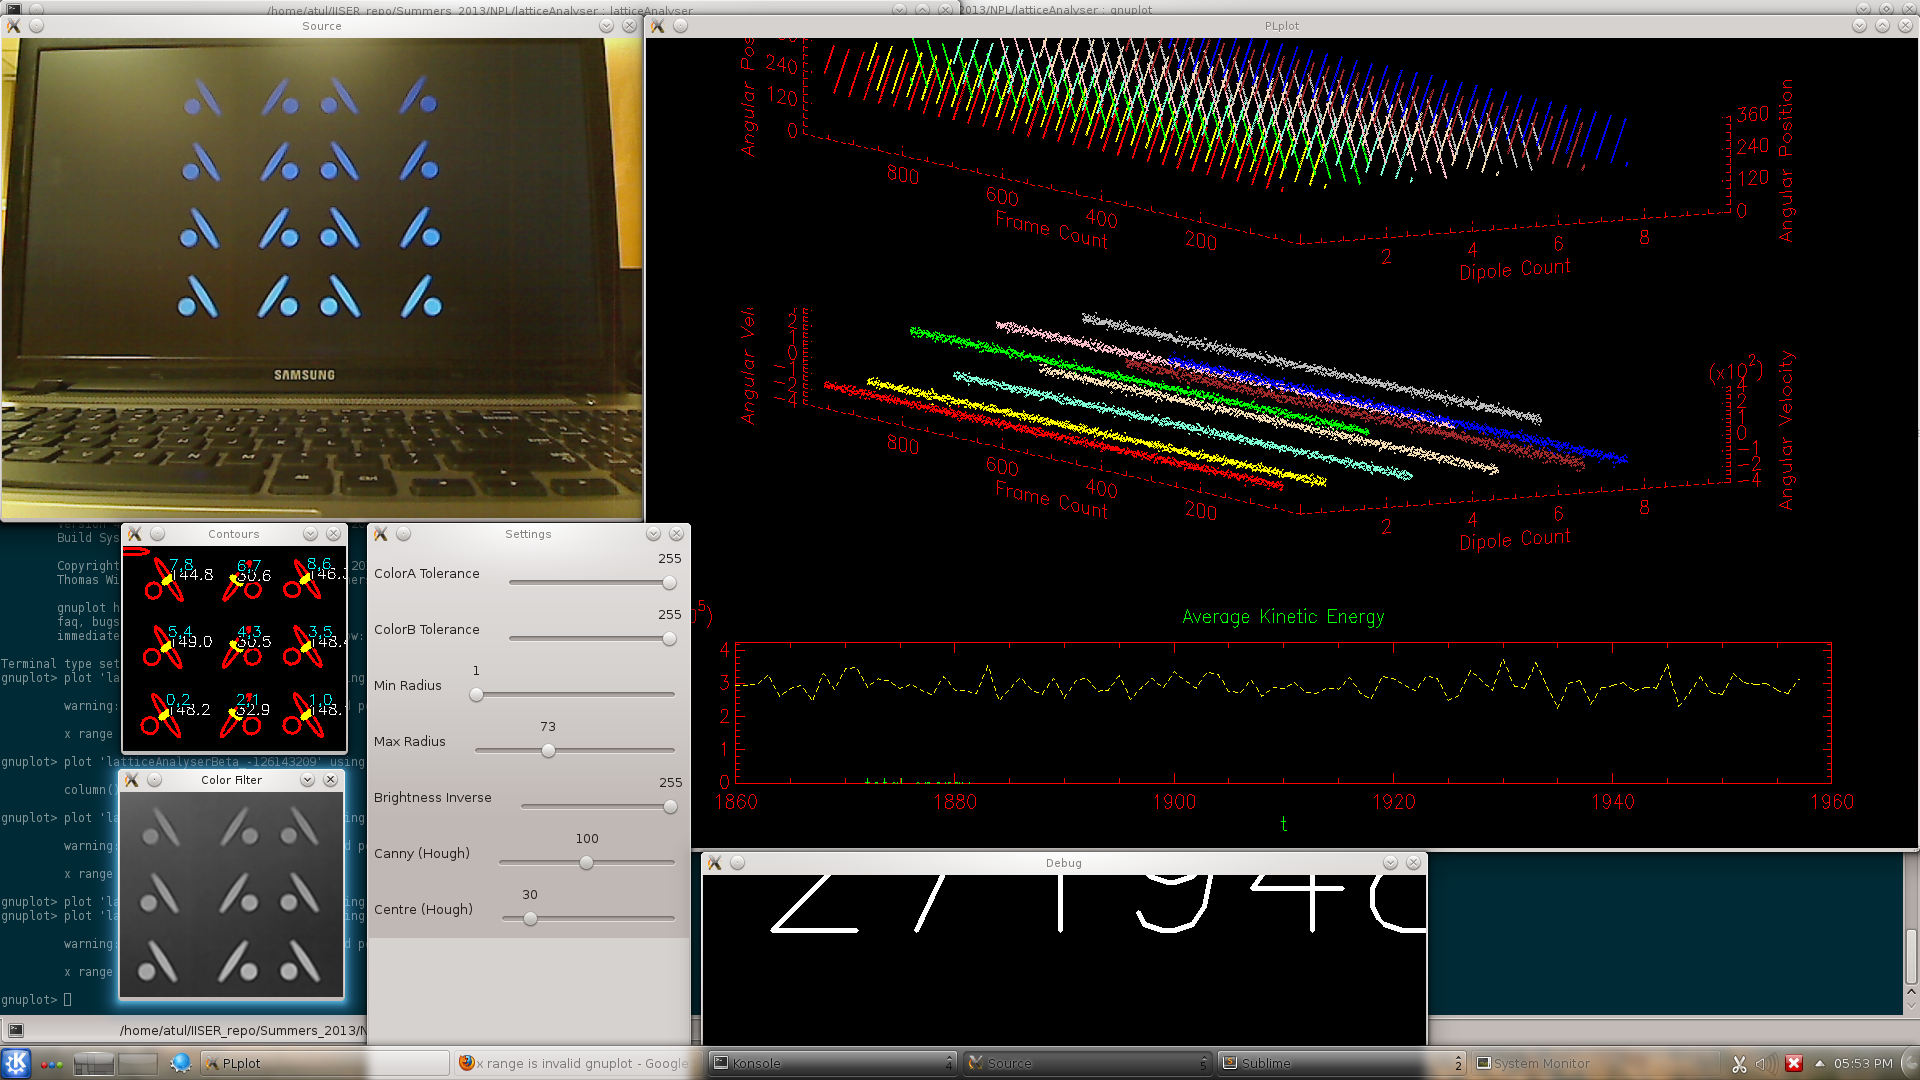
\includegraphics[width=1.1\linewidth]{../../latticeAnalyser/snapshot11.png}
				\end{center}
			\caption[All the three graphs]{All the three graphs}
			\label{snapshot11}
			\end{figure}
			This will probably be the final user interface improvement for the Lattice Analyser.
		\subsubsection{The Modding Problem}
			Consider an ellipse. To describe all its orientations uniquely, given it's position, we need a convention for defining the angle and the angle should span pi radians. Only $\pi$ radians are required as opposed to $2\pi$ simply because of the symmetry of the ellipse. TODO: Put an image of an ellipse with the angle. We therefore need more information than the angle of the ellipse, to determine the angle of the dipole. The design of the pattern takes care of it by providing a circle to break the symmetry. Simplistically, the problem is now solved, for the circle's position can easily be used to decide when to add $\pi$ to the ellipse angle and you have the dipole's angle. TODO: Add an image showing the ellipse with a circle and the dipole angle changed accordingly.
			\par
			Upon implementing this simple logic as an algorithm and testing, it was found that it runs into troubles very quickly and periodically. To understand, first assume that the ellipse reads zero degrees when horizontal and thus, the circle, if it is above the 
			\par
			atan2 approximation for correcting the angle problem, atan2 assisted angle approximation, modular arithmetic based approach for correcting the dipole angle detection (figured this from a simpler problem of firing the elctromagnet)
		\\
		mod problem for deciding when to fire the electro magnet, used modular arithmetic
		\\
		RGB based colour detection to HSV based colour filtering, to improve high speed performance | various problems such as conversion of rgb to hsv and so on..
		\\
		misc: cmake was fiddled around with, auto numbering of lattice points, writing all the data into a file, gstreamer plugins for reading x264
		\\
		graph for kinetic energy added, there was a periodic shoot up, caused by modding problem
		\\
		testing source of systematic error, eliminating a cause, camera defect | calibration. list the two kinds of defects
		\par				
		PHYSICS:
		error analysis: used a lot of GNUplot, to test the kind of deviations for a given dipole, in the angle determination when static, when moving. Then for a given point of time, the deviation in the angles of various dipoles. damping could be tested with realtime grpahs

		Following is the source code of the same, which has been made available online.
		% \lstset{basicstyle=\footnotesize}
		\lstinputlisting[language=C++,title=latticeAnalyser.cpp]{../../latticeAnalyser/latticeAnalyser.cpp}
	\subsection{temperature; the rise}
		`temperature' was built around the Atmega8 processor to start with. It's task was to energize the coils of the dipoles, when instructed by the Lattice Analyser. It's source code was written in C, compiled with the free AVR-GCC compiler using some other sister tools of it. Atmega's interface to the computer was built from \myProf's library, which was built to simplify the existing ob-dev's virtual USB libraries. The coils are powered directly using the chip for the $2\times 2$ setup. For larger matrices, a multiplexer will be required and built suitably.
		\par
		The current that was roughly enough to align the dipole to the coil was (after experiments with a 6 Volt battery and resistance of coil measurement, viz. 7 ohms) found to be about 1 ampere. The microcontroller can sync at most 20 mA of current at a given pin. Further for the USB interface, the system was set to run at 3.3 V (this can be pushed up to 5V also, but that would've required redesigning the circuit) and the current limiting resistor was correspondingly chosen to be about 150 ohms. This was put in series with the coil and tested. It was found that the dipole wouldn't, for even a second long pulse, align itself to the coil, starting from some initial angle. However, when further experiments were done for pumping in energy using the algorithms developed for the Lattice Analyser, this push was found to be enough, even with a few milliseconds long pulse. This version of temperature has been given in \autoref{temperatureFirstVersion}
		\par
		\begin{figure}[bth]
			\begin{center}
				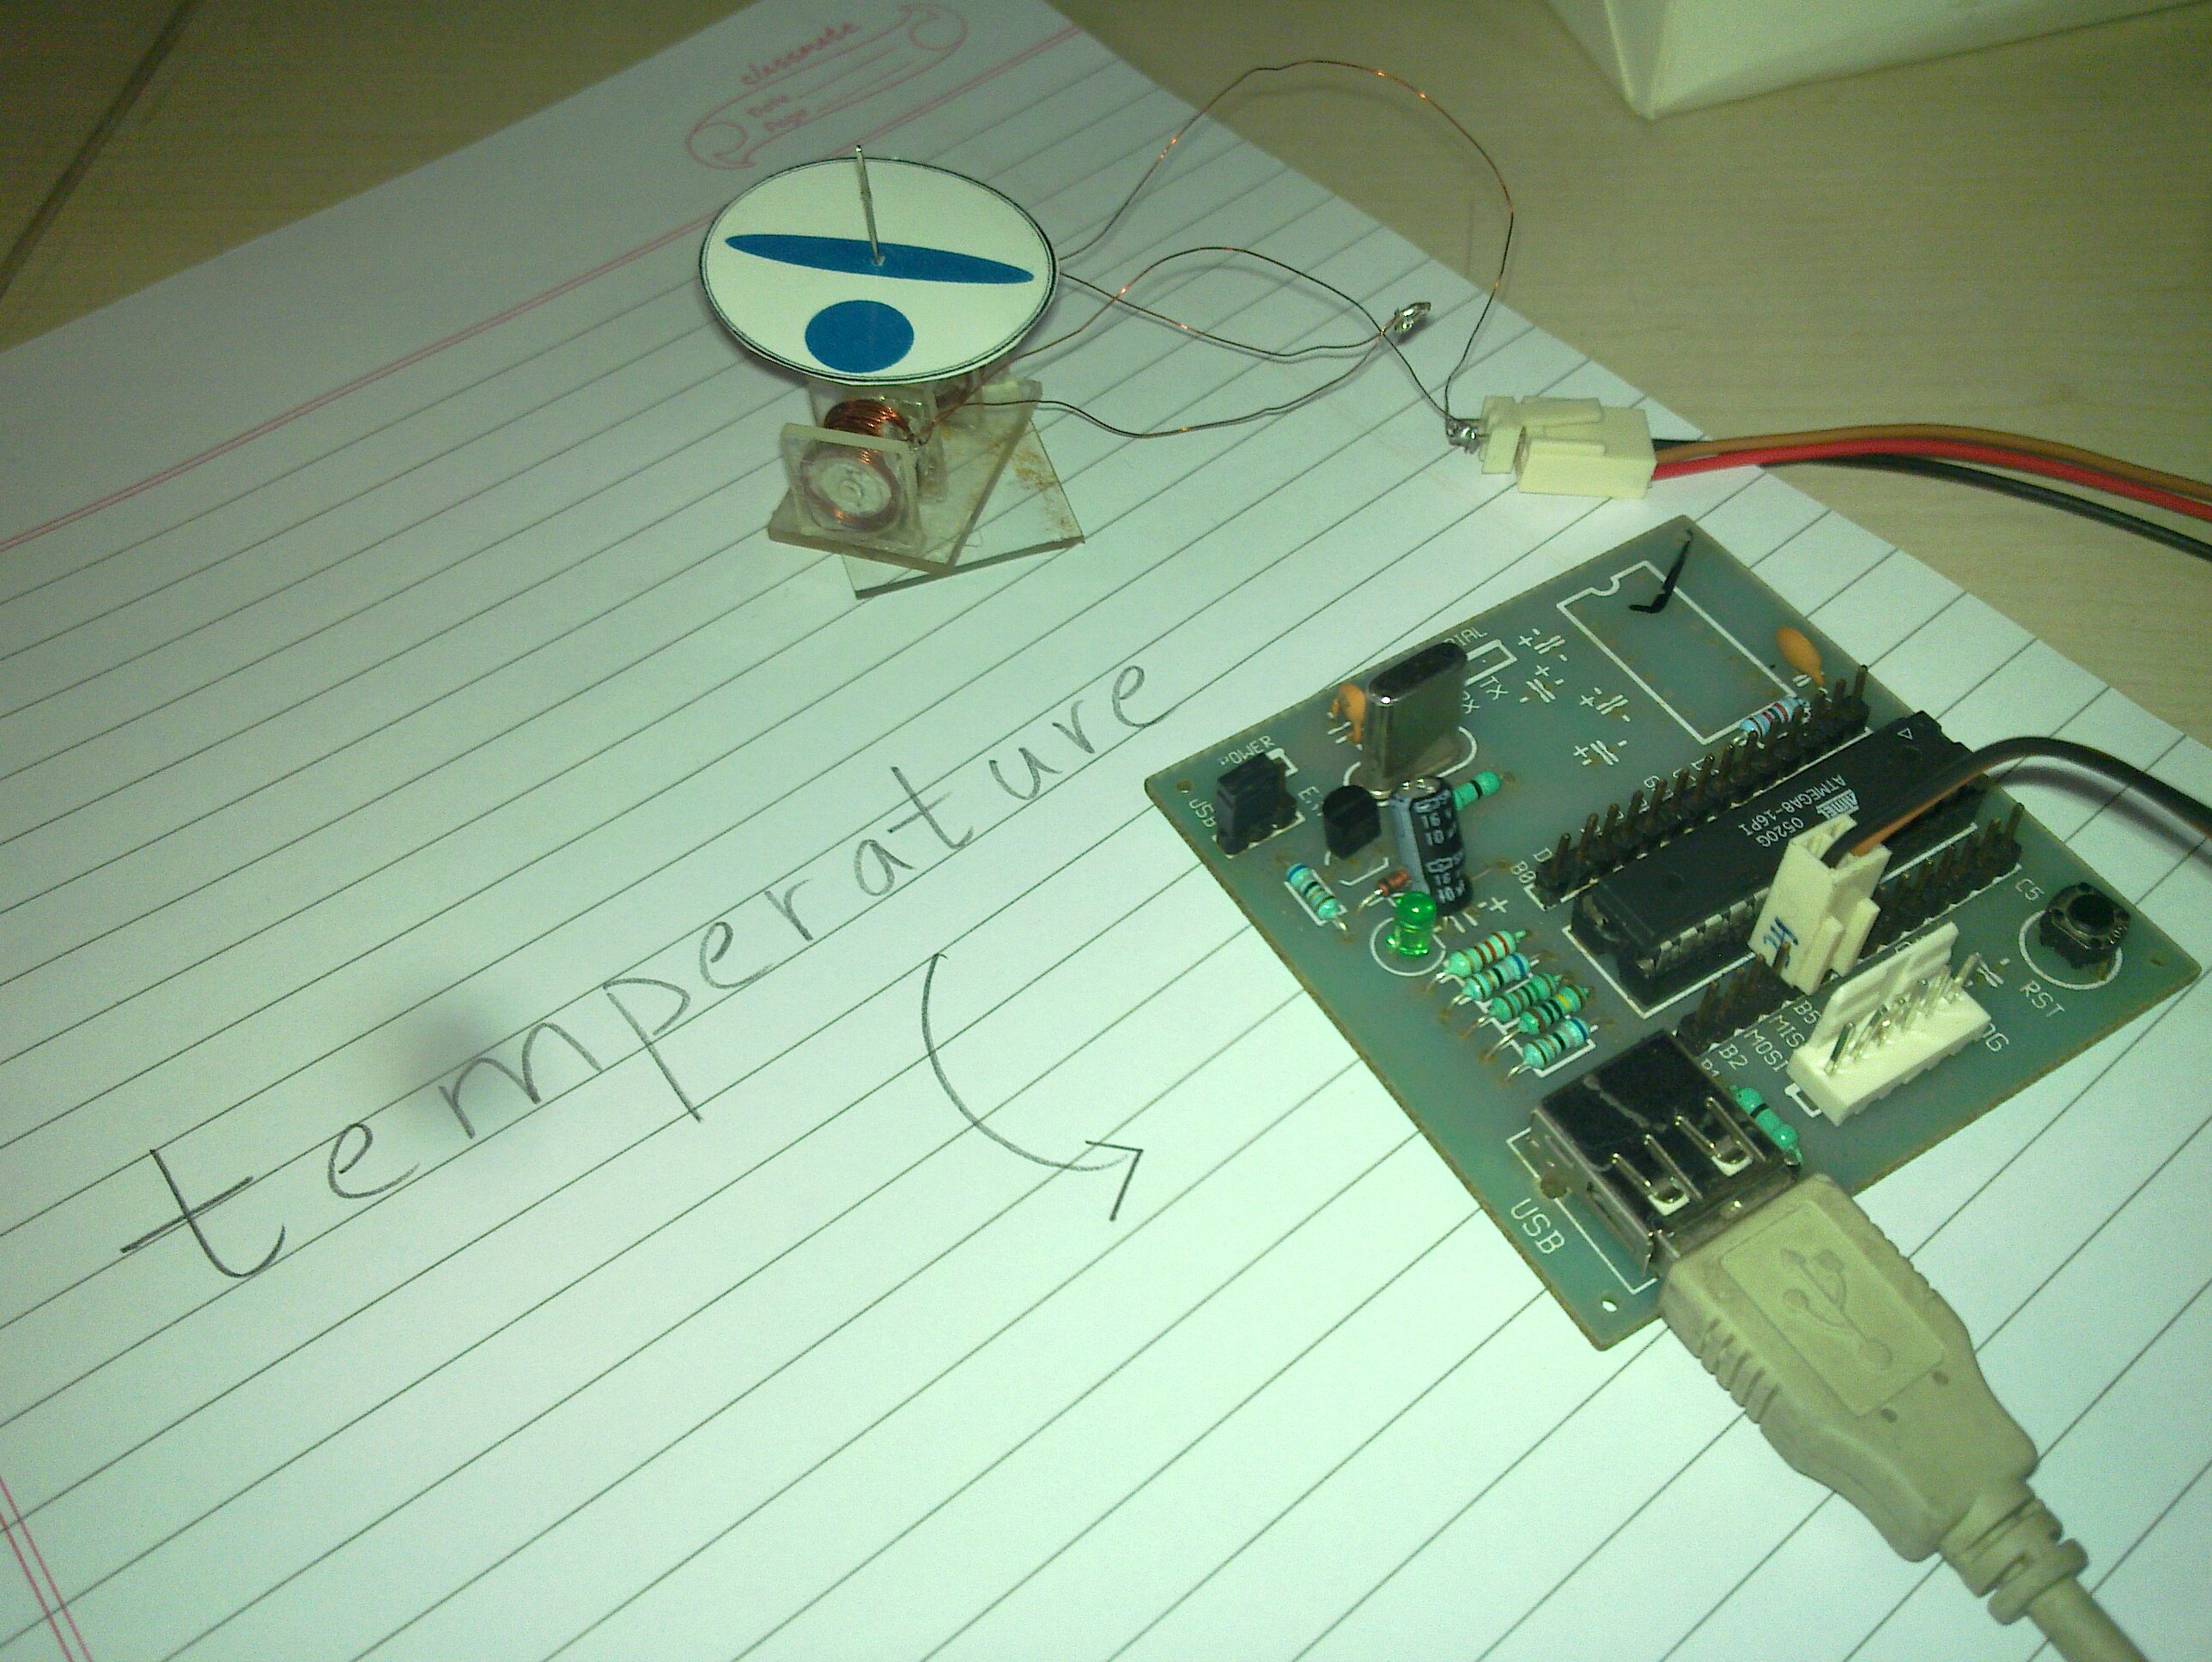
\includegraphics[width=0.85\linewidth]{gfx/temperature.jpg}
			\end{center}
		\caption[First Version of Temperature]{First Version of Temperature}
		\label{temperatureFirstVersion}
		\end{figure}
		\par
		The main file for the temperature has been listed herewith.
		\lstinputlisting[language=C,title=tempereture.c]{../../temperature/firmware/temperature.c}
		\begin{lstlisting}
commit 8e385842ed187496bb320697afceea6ac735183f
Author: Atul Sinh Aurora <toatularora@gmail.com>
Date:   Thu Jul 18 22:23:15 2013 +0530

    Updating the documentation

commit 3fd0c2734e2cb00eaf4e036dee732ff0c38dfca7
Author: Atul Singh Arora <toatularora@gmail.com>
Date:   Tue Jul 16 17:28:58 2013 +0530

    Minor change, major fix (hopefully) fixed the modding problem (after rediscovery:P)

commit 6e6bf4f59a34b0e14246fd8e28845bdc2de401df
Author: Atul Singh Arora <toatularora@gmail.com>
Date:   Tue Jul 16 17:09:45 2013 +0530

    Converted colour detection to HSV from BGR

commit ce55da42951066b207320efe944169b50b82ab08
Author: Atul Singh Arora <toatularora@gmail.com>
Date:   Tue Jul 16 11:40:47 2013 +0530

    Slight failures in the modding problem also resolved..finally based on equivalent classes from math

commit a974f4c3b2aa02e06c3f7df8a6fad2fdd0f66223
Author: Atul Singh Arora <toatularora@gmail.com>
Date:   Tue Jul 16 11:02:29 2013 +0530

    Temperature: SOlved the modding problem for the axis

commit 33fda35ce344b612b786853b044e2229811fefcf
Author: Atul Singh Arora <toatularora@gmail.com>
Date:   Thu Jul 11 15:44:37 2013 +0530

    Completed addition of distortion correction and it has worked well, but hasn't solved the problem

commit 7ad448b39f301eceb69a8bdb1206c67f8f8196ca
Author: Atul Singh Arora <toatularora@gmail.com>
Date:   Thu Jul 11 12:48:02 2013 +0530

    Documentation: README updated

commit 3efc849a25294a881bf05e99af4afa02d6031e2c
Author: Atul Singh Arora <toatularora@gmail.com>
Date:   Wed Jul 10 18:05:57 2013 +0530

    More error analysis and found an error in the error analysis

commit 25debdf7a1a06aeab24b14f66eb597eda39ff7d9
Author: Atul Singh Arora <toatularora@gmail.com>
Date:   Tue Jul 9 17:39:49 2013 +0530

    Doing error analysis on the observations from the software to figure out what to optimize next

commit e2e8270db661e3e902626f188f32d1950445b404
Author: Atul Singh Arora <toatularora@gmail.com>
Date:   Tue Jul 9 12:01:56 2013 +0530

    Ready for error analysis, recorded all the data into a data file

commit 0f8893ca05b450d67c3a23ade21c6d74c693149a
Author: Atul Singh Arora <toatularora@gmail.com>
Date:   Mon Jul 8 17:42:23 2013 +0530

    minor or no change

commit 5c26dd130980019fa34f5700cc5512ddb80d60c7
Author: Atul Singh Arora <toatularora@gmail.com>
Date:   Mon Jul 8 15:24:19 2013 +0530

    latticeAnalyser: Functionality for re-assigning dipole numbers made functional :P

commit 55ea71e74a5416dd7f74171acf7ea1d1ff48d754
Author: Atul Singh Arora <toatularora@gmail.com>
Date:   Mon Jul 8 14:09:03 2013 +0530

    latticeAnalyser: Another finer improvement on the inst vel calculation

commit 6ed09058eb15263ae4ba74775f9b4cafafd9bc83
Author: Atul Singh Arora <toatularora@gmail.com>
Date:   Mon Jul 8 11:23:12 2013 +0530

    Documentation: README updated

commit 1c822e7fe983d18e84be3e3ebe9a8c084ab72f16
Author: Atul Singh Arora <toatularora@gmail.com>
Date:   Fri Jul 5 17:49:41 2013 +0530

    Angle modding problem finally resolved for the greater good :P

commit f83f81c76577417bef7725a040eb638f66a7906d
Author: Atul Singh Arora <toatularora@gmail.com>
Date:   Fri Jul 5 17:12:24 2013 +0530

    Error message in graph; its cause has been resolved and consequently they've been suppressed

commit 35fde5f24b524bc4bcb5ccbd9ad6a72608ed7f54
Author: Atul Singh Arora <toatularora@gmail.com>
Date:   Fri Jul 5 17:38:25 2013 +0530

    Multi threading now functional, though unstable, angle estimator still troublesome, blips

commit 9bda4ff89f6c343609f7a9be0a95d784a8b021c2
Author: Atul Singh Arora <toatularora@gmail.com>
Date:   Fri Jul 5 15:16:45 2013 +0530

    Control for min Angular velocity (for use with temperature) added. Angle estimator now even more stable. No glitches so far

commit 03154549ee38e6b4421f0a27797c4c00dc9626e7
Author: Atul Singh Arora <toatularora@gmail.com>
Date:   Fri Jul 5 14:27:20 2013 +0530

    Angle estimator now more stable, though still gives fluctuations

commit aa67fe4b451af9af9a12acb899e6d28c2e1359cc
Author: Atul Singh Arora <toatularora@gmail.com>
Date:   Fri Jul 5 14:05:55 2013 +0530

    Angle estimator now much more stable, but still peaks out

commit a0dfdae7cda0a9e35b90632d3513ab5a293be6fe
Author: Atul Singh Arora <toatularora@gmail.com>
Date:   Fri Jul 5 13:49:14 2013 +0530

    Angle estimator tested, poor precision with atan2, now using atan2 assisted modding to ellipse based angle detection

commit c515d301935b620fcc2004f5057c63a9881e1974
Author: Atul Singh Arora <toatularora@gmail.com>
Date:   Thu Jul 4 18:23:17 2013 +0530

    Documentation: Screenshot was missed out

commit 9f0faf13c588cbd325a2067f0c54005bdb9f0fe7
Author: Atul Singh Arora <toatularora@gmail.com>
Date:   Thu Jul 4 18:21:42 2013 +0530

    Documentation: README updated

commit a5880c4b1185ed0e5557d51181e3165e8345a7ce
Author: Atul Singh Arora <toatularora@gmail.com>
Date:   Thu Jul 4 18:14:21 2013 +0530

    Kinetic Energy graph added, problem located and calculation corrected

commit 10d125df11fbd250ee3a04e2d51a8bde97cd3f87
Author: Atul Singh Arora <toatularora@gmail.com>
Date:   Wed Jul 3 17:07:57 2013 +0530

    Documentation: Readme updated

commit 3b8a0fcb44b4be72622fb8bff6d7c226a60da80f
Author: Atul Singh Arora <toatularora@gmail.com>
Date:   Wed Jul 3 16:21:51 2013 +0530

    Documentation: READMEs updated

commit 16438bd90783665801e5f334421863af78544773
Author: Atul Singh Arora <toatularora@gmail.com>
Date:   Wed Jul 3 16:19:25 2013 +0530

    Added auto clear on overflow for the graphs

commit a37c4fdb0fce9d140c7ab2e169270392b46daf26
Author: Atul Singh Arora <toatularora@gmail.com>
Date:   Wed Jul 3 15:19:39 2013 +0530

    atan2 used for angles; problem of outlying angles solved

commit 132b1d4b32c794b9bca31ff575521290e30f67fd
Author: Atul Singh Arora <toatularora@gmail.com>
Date:   Wed Jul 3 15:00:05 2013 +0530

    2 graphs in one created, one for velocity, one for position

commit 282c04b3bd3824e77e6d57dcac5f393f2adbf988
Author: Atul Singh Arora <toatularora@gmail.com>
Date:   Wed Jul 3 11:48:52 2013 +0530

    3D graph plotting, updated to show angles

commit 8dedf79959fcb26c39e1ff7c0ec334fc8bf65732
Author: Atul Singh Arora <toatularora@gmail.com>
Date:   Tue Jul 2 17:07:12 2013 +0530

    Fagocytosis successful: Graphing including within the program

commit 5dee7e255f4ac1f281399937619af5db8c012a80
Author: Atul Singh Arora <toatularora@gmail.com>
Date:   Tue Jul 2 16:59:56 2013 +0530

    Fygocytosis done, implementing the rest of it

commit be11592758b03ab9487ffe985ee8de45005db691
Author: Atul Singh Arora <toatularora@gmail.com>
Date:   Tue Jul 2 15:47:53 2013 +0530

    Realtime update finally done for 3d graphics

commit a91a624ccfe896b9acfddd2efbeb24fc5b5d3b24
Author: Atul Singh Arora <toatularora@gmail.com>
Date:   Tue Jul 2 13:59:37 2013 +0530

    Now stable

commit bdcc662088707dd91789a53748d49fee1bef1d76
Author: Atul Singh Arora <toatularora@gmail.com>
Date:   Tue Jul 2 13:52:33 2013 +0530

    Working on using plplot and tried to write an algorithm to support auto grid numbering; but doomed

commit 7c8f275d2e1059b25e33fc34d381a74ed54a3e8e
Author: Atul Sinh Aurora <toatularora@gmail.com>
Date:   Mon Jul 1 11:28:29 2013 +0530

    After summer school

commit 4b1a5a3758caa379c2cdbc2a7e9e657953b5757a
Author: Atul Sinh Aurora <toatularora@gmail.com>
Date:   Sat Jun 8 00:00:05 2013 +0530

    Documentation: code listings updated

commit 261de8437cfc18f8f11d61964343d8529603aa1c
Merge: 803d298 502f050
Author: Atul Sinh Aurora <toatularora@gmail.com>
Date:   Fri Jun 7 23:57:40 2013 +0530

    Merge branch 'master' of https://github.com/toAtulArora/IISER_repo

commit 803d2984bea33f8fb0e206a2f378638048ec90b6
Author: Atul Sinh Aurora <toatularora@gmail.com>
Date:   Fri Jun 7 23:57:06 2013 +0530

    Documentation: Progress for the week added, including the milestone event

commit 502f050adf2d40f697e70b318a8f3705e8837020
Author: Atul Singh Arora <toatularora@gmail.com>
Date:   Fri Jun 7 18:02:18 2013 +0530

    [MileStone commit] latticeAnalyser and temperature: Sight based energy pumping into the dipole successfull

commit 2a24425f8af44d372d9a5b3887c0db0b7aa9989b
Author: Atul Sinh Aurora <toatularora@gmail.com>
Date:   Fri Jun 7 09:00:04 2013 +0530

    latticeAnalyser: trying to compile on windows

commit ae2c44716c144a80ce276959cdae2df1a92856bf
Author: Atul Sinh Aurora <toatularora@gmail.com>
Date:   Thu Jun 6 16:24:23 2013 +0530

    sachetIO: buffer function fixed and tested ok

commit efa7bdded264e2aeb81945a807e975637ae8e47a
Author: Atul Sinh Aurora <toatularora@gmail.com>
Date:   Thu Jun 6 15:32:22 2013 +0530

    sachetIO: added the buffered read function

commit 22b0d4a24d5281dd1753aba4ab1b6a71b341bf7d
Author: Atul Sinh Aurora <toatularora@gmail.com>
Date:   Thu Jun 6 13:21:03 2013 +0530

    Documentation: Readme Updated with Wednesday's progress

commit ffcc38dffd780bb33e426f323e42626cd5db1f6b
Author: Atul Sinh Aurora <toatularora@gmail.com>
Date:   Wed Jun 5 22:42:27 2013 +0530

    sachetIO: bare minimum fixed and tested

commit ea3e045f05988e42d9eb2dd884a3ceff949e4abc
Author: Atul Sinh Aurora <toatularora@gmail.com>
Date:   Wed Jun 5 21:45:36 2013 +0530

    sachetIO: Fixing recieving

commit 07b8135ddeeed04430704625bc95cc3091d2098a
Author: Atul Sinh Aurora <toatularora@gmail.com>
Date:   Wed Jun 5 21:13:32 2013 +0530

    sachetIO: Sending tested

commit 0cb0ee0d725288a914cdc7327b7d8271a4545a13
Author: Atul Sinh Aurora <toatularora@gmail.com>
Date:   Wed Jun 5 20:46:09 2013 +0530

    Debugging sachetIO

commit a0e26da38bc55571ae426e30f820aa3b83c0aa8a
Author: Atul Sinh Aurora <toatularora@gmail.com>
Date:   Wed Jun 5 18:55:06 2013 +0530

    lattice and temperature: sachetIO added, not tested

commit 91ad9c62158050abf17d2845df6a73e459bd6dc6
Author: Atul Sinh Aurora <toatularora@gmail.com>
Date:   Wed Jun 5 11:13:13 2013 +0530

    Windows thumbnail updated, bad gitting

commit 971107d27875483c7da099fbc919bb3ff6e10cbc
Author: Atul Singh Arora <toatularora@gmail.com>
Date:   Tue Jun 4 17:38:28 2013 +0530

    Documentation: Readme updated

commit 1ae6231a7947ff2dfb60cde8c5ff6f04126fe6dd
Author: Atul Singh Arora <toatularora@gmail.com>
Date:   Tue Jun 4 17:17:29 2013 +0530

    latticeAnalyser: Brightness level added amongst other mods

commit 66e0a71c8883402d9f417ceee81fd90aae6b3978
Merge: 5197b0e f74225f
Author: Atul Singh Arora <toatularora@gmail.com>
Date:   Tue Jun 4 16:29:11 2013 +0530

    Sync between i7 and the laptop i3.

commit f74225f45621d6787eabb6aa8f1a6b8b2a2ed838
Merge: a9e3f77 0acd87a
Author: Atul Sinh Aurora <toatularora@gmail.com>
Date:   Tue Jun 4 16:25:39 2013 +0530

    Merge branch 'master' of https://github.com/toAtulArora/IISER_repo

commit a9e3f773ce60d4d2208df7916ded4eb265dc3374
Author: Atul Sinh Aurora <toatularora@gmail.com>
Date:   Tue Jun 4 16:25:00 2013 +0530

    Dipoles for printing corrected

commit 5197b0e7cdf547ab1f2d0ac919d75a7374091b18
Author: Atul Singh Arora <toatularora@gmail.com>
Date:   Tue Jun 4 16:19:24 2013 +0530

    Completed Firing the electro using the console

commit 61a7d99bbaca3a1ff5bd242605a5d02931189fb1
Author: Atul Singh Arora <toatularora@gmail.com>
Date:   Tue Jun 4 12:28:48 2013 +0530

    Protocol tested | functional

commit d216f3253d72c34b41a37c3de40d3de4c7e4df61
Author: Atul Singh Arora <toatularora@gmail.com>
Date:   Tue Jun 4 12:10:52 2013 +0530

    lattice and temp, both about to be tested

commit 1c300638b1a4f72d4bd0c1adc871aa4e331f604a
Author: Atul Sinh Aurora <toatularora@gmail.com>
Date:   Tue Jun 4 11:44:14 2013 +0530

    Dipoles for printing prepared

commit 5716ed3aac119b7f9ed73fdf91fd3cc5d582f3ad
Author: Atul Singh Arora <toatularora@gmail.com>
Date:   Tue Jun 4 10:20:38 2013 +0530

    temperature: modifying directory structures

commit 0acd87a44061dbad55c16cdaf3edeb83f0ba282e
Author: Atul Singh Arora <toatularora@gmail.com>
Date:   Tue Jun 4 10:12:00 2013 +0530

    Committing missed out changes

commit bc84259a0622c96483cd2a2e6192c64a50001387
Author: Atul Singh Arora <toatularora@gmail.com>
Date:   Tue Jun 4 10:10:06 2013 +0530

    Improving makefiles

commit 41bf3439997260e2ea985159dbeac26f3c932e09
Author: Atul Singh Arora <toatularora@gmail.com>
Date:   Tue Jun 4 09:59:29 2013 +0530

    latticeAnalyser and temperature: Now test built and stable together

commit 87e256921410d3b3dd64d3cf5c7bee2a07f2d07c
Author: Atul Singh Arora <toatularora@gmail.com>
Date:   Mon Jun 3 18:25:20 2013 +0530

    Unstable: Testing temperature with latticeAnalyser

commit 414bd316aee99f833fb0990d46ed8e8e812bb431
Author: Atul Singh Arora <toatularora@gmail.com>
Date:   Mon Jun 3 16:22:39 2013 +0530

    Completed making a directory structure and compiling with a makefile, the original program. Plus brought the latticeAnalyser up to pace, ready to be tested with a makefile

commit 45870e0b999e2a2fb5262c1724524c32344146e0
Author: Atul Singh Arora <toatularora@gmail.com>
Date:   Mon Jun 3 15:11:22 2013 +0530

    temperature: Brought to life

commit 45ec731b3acdd2453b9b398f2bab241f44a1d44c
Author: Atul Sinh Aurora <toatularora@gmail.com>
Date:   Mon Jun 3 09:06:32 2013 +0530

    Documentation: Minor changes

commit c9dba8a5a11417bcd88e5871d21447634d8dcdf8
Author: Atul Sinh Aurora <toatularora@gmail.com>
Date:   Sun Jun 2 21:21:18 2013 +0530

    Documentation: Report completed for this week

commit a8caec9bc8d48e292500a67aaa4ab30307ce5f3c
Author: Atul Sinh Aurora <toatularora@gmail.com>
Date:   Sun Jun 2 20:23:22 2013 +0530

    Documentation: Updating the report, air levitation bit

commit 81911d7db6ad61c78adb43cdf38f923463e99ea2
Author: Atul Sinh Aurora <toatularora@gmail.com>
Date:   Sun Jun 2 13:59:47 2013 +0530

    Tested and functional in windows

commit 545b4b2a6f2fe5b479b2b195db3e33bf07dcbd05
Author: Atul Singh Arora <toatularora@gmail.com>
Date:   Fri May 31 17:49:46 2013 +0530

    Documentation: Updating the readme with todays update

commit 6ba72ab3722dde5108c24f36cf1f0b7a431a5473
Author: Atul Singh Arora <toatularora@gmail.com>
Date:   Fri May 31 17:47:33 2013 +0530

    latticeAnalyser: Working on the CLI to support hardware test and interface

commit c02f28b3cb63b80de999d6e48caf7d1c11ee134b
Merge: e799380 4124d6f
Author: Atul Singh Arora <toatularora@gmail.com>
Date:   Fri May 31 09:37:56 2013 +0530

    Merge between my laptop on the i7

commit 4124d6f02088e68eee26a717a2d311d878e94e14
Merge: e7fdc40 b9fa975
Author: Atul Sinh Aurora <toatularora@gmail.com>
Date:   Fri May 31 09:37:40 2013 +0530

    Merge branch 'master' of https://github.com/toAtulArora/IISER_repo

commit e79938071a4774aead45190065d4b89ec897f172
Author: Atul Singh Arora <toatularora@gmail.com>
Date:   Fri May 31 09:36:41 2013 +0530

    Documentation: Readme updated

commit e7fdc40f167da5cc37e4be6d00126a16139b6392
Author: Atul Sinh Aurora <toatularora@gmail.com>
Date:   Fri May 31 09:35:45 2013 +0530

    latticeAnalyser: Working on adding hardware support

commit b9fa9750312fbd712d4f67e412c6f8fa439d2e3f
Author: Atul Singh Arora <toatularora@gmail.com>
Date:   Thu May 30 14:48:47 2013 +0530

    Documentation: Updating the readme

commit e5ab8b0d86d65f425b6cb8882fe2e3e217ef32f8
Merge: 96497a8 8641fbb
Author: Atul Sinh Aurora <toatularora@gmail.com>
Date:   Thu May 30 11:14:22 2013 +0530

    Merge branch 'master' of https://github.com/toAtulArora/IISER_repo

commit 8641fbb08ea2310ef683cf273e246372083ca0fd
Merge: 947f4a9 eb3aa7b
Author: Atul Singh Arora <toatularora@gmail.com>
Date:   Thu May 30 12:03:26 2013 +0530

    Merge remote-tracking branch 'origin'

commit 947f4a92fdb40167b79fbcbf0703961068e9d928
Author: Atul Singh Arora <toatularora@gmail.com>
Date:   Thu May 30 12:03:04 2013 +0530

    Documentation: For installing the avr tool chain added

commit 96497a8bfdaa355470b28457c0c3258e58246727
Author: Atul Sinh Aurora <toatularora@gmail.com>
Date:   Thu May 30 11:13:55 2013 +0530

    Testing Air Levitation: Drawing for drilling corrected

commit eb3aa7ba02b8fe4e8fe461a1fcf3f48985637ac7
Author: Atul Sinh Aurora <toatularora@gmail.com>
Date:   Thu May 30 11:01:53 2013 +0530

    Testing Air Levitation: Drawing for drilling completed

commit 88a86f88320485cf29a4bd549fc596574efb5cd7
Author: Atul Singh Arora <toatularora@gmail.com>
Date:   Wed May 29 18:18:42 2013 +0530

    Compiled with linux, gcc and opencv built with openTBB and IPP, in i7, seems to be screeching fast so far

commit 97e92d0a1c358a48f6268620e8f27550fe4df930
Merge: a06ca8c 88a86f8
Author: Atul Sinh Aurora <toatularora@gmail.com>
Date:   Wed May 29 17:27:41 2013 +0530

    Merge branch 'master' of https://github.com/toAtulArora/IISER_repo

commit a06ca8c3c46b595a18fd2857b67181a58d426b3c
Author: Atul Sinh Aurora <toatularora@gmail.com>
Date:   Wed May 29 17:27:18 2013 +0530

    Adding the dipole image

commit dd49ef3da14113786804d091524dc9fe985f1ba2
Merge: 7118975 c5783f2
Author: Atul Sinh Aurora <toatularora@gmail.com>
Date:   Tue May 28 17:53:20 2013 +0530

    Resolving conflicts

commit c5783f2c0326b6f9932a79cb1ebcb6423eb5f3f4
Author: Atul Sinh Aurora <toatularora@gmail.com>
Date:   Tue May 28 17:49:26 2013 +0530

    Finalizing, now stable in windows, tested

commit 9094e4956634cf6552d4a13034681c9aa467ced4
Author: Atul Sinh Aurora <toatularora@gmail.com>
Date:   Tue May 28 17:40:52 2013 +0530

    Multi-Thread Atomic Sync Completed to satisfactory level

commit 54ef6c6562e5191d9a13fc28f4af5bb86aa0d9b8
Author: Atul Sinh Aurora <toatularora@gmail.com>
Date:   Tue May 28 17:12:15 2013 +0530

    Display atomic multi-thread, mysteriously functional

commit aea12d12ff7a7392a9a8aa6bfc24b9480fac2bed
Author: Atul Sinh Aurora <toatularora@gmail.com>
Date:   Tue May 28 16:10:41 2013 +0530

    Atomic Sync implemented for capture frame

commit 4c37bfb7a65726b0c5d4c0be78efa8adf308db20
Author: Atul Singh Arora <toatularora@gmail.com>
Date:   Tue May 28 15:22:27 2013 -0800

    Working on atomic aspects. Now switching to visual studio

commit ec9f99c1950c6590f14f011b5ced221a71bb44a4
Author: Atul Singh Arora <toatularora@gmail.com>
Date:   Tue May 28 11:18:46 2013 -0800

    Working on the multithreaded aspect, somehow still faster without multithreading

commit 7118975120137a637efbdfd00f4f37029dcb48f5
Author: Atul Sinh Aurora <toatularora@gmail.com>
Date:   Tue May 28 15:37:55 2013 +0530

    Minor changes

commit 1937a9b1a85d298adf71082c7d4d5d0b2e2459ed
Author: Atul Singh Arora <toatularora@gmail.com>
Date:   Mon May 27 16:58:04 2013 -0800

    Support for multi-threading added, also compiled with IPP

commit 634469581390949623305417360e3337e2c4b559
Author: Atul Singh Arora <toatularora@gmail.com>
Date:   Mon May 27 11:40:47 2013 -0800

    Multi threaded for reducing lag

commit 118b1118a3a9c9a2450c97857dfa1f3c7cdce17a
Author: Atul Sinh Aurora <toatularora@gmail.com>
Date:   Thu May 23 15:42:56 2013 +0530

    Template Record modified and commited

commit b15b3b68ecf14b8f6412e68a0e32e07fafb8b320
Author: Atul Sinh Aurora <toatularora@gmail.com>
Date:   Thu May 23 14:17:21 2013 +0530

    Template Record zip added

commit 69cc3d0baf0c5593220504d6184379cf4f1eeaac
Author: Atul Sinh Aurora <toatularora@gmail.com>
Date:   Thu May 23 14:16:29 2013 +0530

    Adding the template amongst other things

commit 65be7489adf56a9d1ddb5429a812446b6d5a90fe
Author: Atul Sinh Aurora <toatularora@gmail.com>
Date:   Tue May 21 21:07:12 2013 +0530

    Minor bug, memory leak corrected.

commit d491b930c62d39d8d9032d7a7361fc302fccd29e
Author: Atul Sinh Aurora <toatularora@gmail.com>
Date:   Tue May 21 19:25:15 2013 +0530

    Windows Support Added, amongst other things

commit 76de5131ce3281f6a67c6fa4e2e04390eb9ffddf
Merge: 92b9031 5bd296f
Author: Atul Sinh Aurora <toatularora@gmail.com>
Date:   Mon May 20 17:16:48 2013 +0530

    Merge branch 'master' of https://github.com/toAtulArora/IISER_repo

commit 5bd296f6330bc6a994cdd3cb568944ddae03ddd4
Author: Atul Singh Arora <toatularora@gmail.com>
Date:   Mon May 20 17:16:10 2013 -0800

    Corrections

commit 7f19fcacfdd84895a66df61918983d26b9966f5c
Author: Atul Singh Arora <toatularora@gmail.com>
Date:   Mon May 20 14:02:50 2013 -0800

    latticeAnalyser functional again

commit 4720ab5b6ce0310a35c4e67392430d8248b488c4
Author: Atul Singh Arora <toatularora@gmail.com>
Date:   Mon May 20 14:02:04 2013 -0800

    Test results for speed added

commit f546e50310b6a9721430739bd0d1710939d4f98e
Author: Atul Singh Arora <toatularora@gmail.com>
Date:   Mon May 20 12:48:50 2013 -0800

    Testing: Computation time

commit 92b903140f65e1a1dc13fa340d2ba60f467a907d
Merge: 6b87a0b 7f19fca
Author: Atul Sinh Aurora <toatularora@gmail.com>
Date:   Mon May 20 14:03:18 2013 +0530

    Merge branch 'master' of https://github.com/toAtulArora/IISER_repo

commit 6b87a0bea18e78b97272fa4d2948add994f9be0b
Merge: c18ab4f f546e50
Author: Atul Sinh Aurora <toatularora@gmail.com>
Date:   Mon May 20 12:51:15 2013 +0530

    Merge branch 'master' of https://github.com/toAtulArora/IISER_repo

commit c18ab4f832ab6905bd110cb35f97f462ad4d64e3
Author: Atul Sinh Aurora <toatularora@gmail.com>
Date:   Mon May 20 12:51:01 2013 +0530

    Testing Overall speed

commit d902a319f303aa07b7744b28b10c2b7f7d9d4704
Author: Atul Sinh Aurora <toatularora@gmail.com>
Date:   Mon May 20 08:49:51 2013 +0530

    Documentation: Pushing final changes

commit 3961ae759ca5d8cd49ea0fc5b1f117808af64357
Author: Atul Sinh Aurora <toatularora@gmail.com>
Date:   Mon May 20 00:59:40 2013 +0530

    Documentation: For this week, completed

commit 600d76a3c5a0157d2704643c7606a6f4845015a0
Author: Atul Sinh Aurora <toatularora@gmail.com>
Date:   Sun May 19 23:32:05 2013 +0530

    Documentation: Working on it

commit 97dfb751a1e095d12c2bd9b8bfdb692f2c7fc9f8
Author: Atul Sinh Aurora <toatularora@gmail.com>
Date:   Sun May 19 21:33:03 2013 +0530

    Latex documentation initiated

commit 965a960cc01ba8c12828c9c7184002abfa254516
Author: Atul Sinh Aurora <toatularora@gmail.com>
Date:   Sat May 18 21:18:13 2013 +0530

    Documentation: Graph for the result added

commit 2b54dcdccda1674acd1e55b4811deef84af22bd6
Author: Atul Sinh Aurora <toatularora@gmail.com>
Date:   Fri May 17 20:05:53 2013 +0530

    Documentation: Graphs added plus the screenshots fixed

commit b451f3235971d518bdb8b598d7d0617b30d1905c
Merge: 24299e9 e6992b4
Author: Atul Sinh Aurora <toatularora@gmail.com>
Date:   Fri May 17 19:49:02 2013 +0530

    Merge branch 'master' of https://github.com/toAtulArora/IISER_repo

commit e6992b4d4dfdd247e13cc26792e5ae2e967b71e7
Merge: b99fa82 e6a9613
Author: Atul Singh Arora <toatularora@gmail.com>
Date:   Fri May 17 17:29:37 2013 -0800

    Merge branch 'master' of github.com:toAtulArora/IISER_repo

commit b99fa823120154b9605e9c7295f7b1095788940c
Author: Atul Singh Arora <toatularora@gmail.com>
Date:   Fri May 17 17:28:39 2013 -0800

    junk files removed

commit 2f90706321725486350bf5e5cab471880024732c
Author: Atul Singh Arora <toatularora@gmail.com>
Date:   Fri May 17 17:28:05 2013 -0800

    Tested with movement, Passed so far atleast qualitatively

commit d0713d1bc4387bc86ffa97ffa70e7135461c1c8d
Author: Atul Singh Arora <toatularora@gmail.com>
Date:   Fri May 17 16:49:45 2013 -0800

    Data readout successful

commit 9562182c76cdd8bd3332369b077a537979b38226
Author: Atul Singh Arora <toatularora@gmail.com>
Date:   Fri May 17 14:38:46 2013 -0800

    Unstable: working on saving the data in frames

commit 24299e9b82d126498eb9fdb2a423b73dc10c956a
Author: Atul Sinh Aurora <toatularora@gmail.com>
Date:   Fri May 17 17:48:00 2013 +0530

    Completing documentation

commit e6a961387d67fc44b61d9d4a7ff8cdbf3c9300c8
Author: Atul Sinh Aurora <toatularora@gmail.com>
Date:   Fri May 17 17:07:59 2013 +0530

    Test animation added

commit c4b267c3aee1b4a250b35947909b9b66d840e124
Merge: 592f37f e76bdab
Author: Atul Sinh Aurora <toatularora@gmail.com>
Date:   Fri May 17 06:26:55 2013 +0100

    Merge branch 'master' of https://github.com/toAtulArora/IISER_repo

commit e76bdab03a3563f80b2b6a7df35a03cf5016cb08
Merge: c577396 139aa07
Author: Atul Singh Arora <toatularora@gmail.com>
Date:   Fri May 17 10:56:05 2013 -0800

    Merge branch 'master' of github.com:toAtulArora/IISER_repo

commit c5773969054079d95f2b6ffa6374a70bc37edae3
Author: Atul Singh Arora <toatularora@gmail.com>
Date:   Fri May 17 10:55:28 2013 -0800

    Stable and tested, the dipole angle measurement for each frame is successful

commit 1b512fc3f783b9ceab973241bac17de424fcf374
Merge: 17b9e98 7ed3367
Author: Atul Singh Arora <toatularora@gmail.com>
Date:   Fri May 17 10:21:26 2013 -0800

    Merge branch 'master' of github.com:toAtulArora/IISER_repo

commit 17b9e981d3d6eca9e1bcb5057c6e9223615685b0
Author: Atul Singh Arora <toatularora@gmail.com>
Date:   Fri May 17 10:21:09 2013 -0800

    Dipole detection successful and stable

commit 592f37fa548922654bfae0d0df77f873243a1501
Author: Atul Sinh Aurora <toatularora@gmail.com>
Date:   Fri May 17 06:26:44 2013 +0100

    Image Rotated

commit 139aa076a25cb555d7ea8148a5ffc5d16efac3ef
Author: Atul Sinh Aurora <toatularora@gmail.com>
Date:   Fri May 17 10:36:18 2013 +0530

    Dipoles modified, ellipse thinner

commit 7ed336730f865b7fa6dd42b966062c47b12414ce
Author: Atul Sinh Aurora <toatularora@gmail.com>
Date:   Fri May 17 09:51:06 2013 +0530

    Circle Ellipse for Dipole

commit a28114a6da1a2c41eea58773edbe7b36be55bfd1
Author: Atul Sinh Aurora <toatularora@gmail.com>
Date:   Fri May 17 09:17:00 2013 +0530

    STABLE upto mod 180. Updated a few things

commit 71f70879c14c7ee04accd4967eb30efadcfb503b
Author: Atul Sinh Aurora <toatularora@gmail.com>
Date:   Thu May 16 20:01:51 2013 +0530

    Dipole diagrams under development

commit 67091067fca83d9bd6b82435a147fa147b73a9ce
Author: Atul Singh Arora <toatularora@gmail.com>
Date:   Thu May 16 18:30:23 2013 -0800

    Stable and angle detection, Mod PI stable

commit f0331273de52a2cbc08375adf828c8c19c793b5a
Merge: 0a238d6 fbf2852
Author: Atul Singh Arora <toatularora@gmail.com>
Date:   Thu May 16 17:51:57 2013 -0800

    Merge remote branch 'origin'

commit 0a238d683fca9596f1f4e39b476239495fb431a0
Author: Atul Singh Arora <toatularora@gmail.com>
Date:   Thu May 16 17:50:47 2013 -0800

    Stable but not functional, the angle detection

commit fbf2852326d676b5249558b81bd9fb9359f5c050
Author: Atul Sinh Aurora <toatularora@gmail.com>
Date:   Thu May 16 11:23:54 2013 +0530

    Darker

commit 3e35bb152be886098e2ad3c627eb97d655ac4156
Author: Atul Sinh Aurora <toatularora@gmail.com>
Date:   Thu May 16 10:54:22 2013 +0530

    Ellipses, exported

commit 8a77a1cda5fedb8a31384aba38e7f9c59822d7d9
Author: Atul Sinh Aurora <toatularora@gmail.com>
Date:   Thu May 16 10:34:13 2013 +0530

    Ellipses: Dipoles now have ellipses

commit 1352099dd4b874d3c40feeaf1bb60ba2ecc0e0ac
Author: Atul Singh Arora <toatularora@gmail.com>
Date:   Wed May 15 16:46:49 2013 -0800

    Readme fixed

commit d4dde74debd2808ed61985555efed5e3f249faa8
Author: Atul Singh Arora <toatularora@gmail.com>
Date:   Wed May 15 16:45:34 2013 -0800

    latticeAnalyser now Stable

commit 8185f26452a568f24436dad15d7721c6abf09507
Author: Atul Singh Arora <toatularora@gmail.com>
Date:   Wed May 15 15:46:39 2013 -0800

    readme fix

commit b5c2f8ef6f30b41f8922595de45b2d21078ee535
Author: Atul Singh Arora <toatularora@gmail.com>
Date:   Wed May 15 15:45:36 2013 -0800

    readme fix

commit a1882f5b9ca8608c5f5078959990de0f4328d0af
Author: Atul Singh Arora <toatularora@gmail.com>
Date:   Wed May 15 15:44:17 2013 -0800

    Proof of concept for Hough

commit c4c85189bc2a33a21fa4bd18e746d5faff8f4cc3
Author: Atul Singh Arora <toatularora@gmail.com>
Date:   Wed May 15 14:54:41 2013 -0800

    Proof of concept is complete

commit 7989309295af080c63d2359e228548a83df384f0
Author: Atul Singh Arora <toatularora@gmail.com>
Date:   Wed May 15 14:32:34 2013 -0800

    Test version functional with contours, for circle detection

commit 48eb9ca66cd831e7622c3411e5d772dc48861853
Author: Atul Singh Arora <toatularora@gmail.com>
Date:   Wed May 15 13:19:45 2013 -0800

    Test with circles, using contours is fine

commit 38c0db3f5a80f766d6ce392874cfc6dbd0c98084
Author: Atul Sinh Aurora <toatularora@gmail.com>
Date:   Wed May 15 13:01:00 2013 +0530

    Plaussibly unstable, rewriting latticeAnalyser

commit ae3ed9a080a08f1293835340bbe27f67bb03a092
Author: Atul Sinh Aurora <toatularora@gmail.com>
Date:   Wed May 15 11:51:55 2013 +0530

    Added the dipole drawing

commit bbcf6834ea3ea5a8bc8beaccc111802da44ac762
Author: Atul Singh Arora <toatularora@gmail.com>
Date:   Tue May 14 16:39:23 2013 -0800

    Readme final update for tuesday

commit 7d37eb031af55077a3406fcb8636be9ff9c50688
Author: Atul Singh Arora <toatularora@gmail.com>
Date:   Tue May 14 14:47:01 2013 -0800

    Updating the readme

commit b468d8f06c6b1ce0a6ab8584c144766bb3c832e6
Author: Atul Singh Arora <toatularora@gmail.com>
Date:   Tue May 14 14:45:57 2013 -0800

    Updating the readme

commit 9050ca5cf5520a743c9fd15b1c62d1a4ebda7e01
Author: Atul Singh Arora <toatularora@gmail.com>
Date:   Tue May 14 14:10:03 2013 -0800

    Trying to push changes

commit 85749c48d6c87e4ae693daff193ff5c6682fe577
Author: root <root@ccf1.ccf.npl>
Date:   Tue May 14 12:58:47 2013 -0800

    Up and running in the new setup

commit b31da232eef661b854d86ea0f495f2f491a74a58
Author: Atul Singh Arora <toatularora@gmail.com>
Date:   Tue May 14 12:51:14 2013 +0530

    Migrating :(

commit a8cbef25fc90a3c878456f921b2a029dd5b0b058
Author: Atul Singh Arora <toatularora@gmail.com>
Date:   Mon May 13 12:09:08 2013 +0530

    Basic Colour Filters up and running

commit 118a3519f5123a64ac8049229462213f02f6052e
Author: Atul Singh Arora <toatularora@gmail.com>
Date:   Mon May 13 11:54:40 2013 +0530

    The lattice analyser is being built..has begun to 'see' things

commit 75bd2af30f3ee056eb2b840877782803f4a8bda5
Author: Atul Singh Arora <toatularora@gmail.com>
Date:   Sat May 11 15:25:51 2013 +0530

    Setting up the structure

commit f3751b794796ddb116da91dbf4d034faec6a5998
Author: Atul Singh Arora <toatularora@gmail.com>
Date:   Sat May 11 13:52:10 2013 +0530

    Readme Updated		
		\end{lstlisting}	